%============================================================
% BAB 4 — hasil konversi awal dari DOCX lama
%============================================================
\chapter{EKSPERIMEN DAN ANALISIS}

Bab ini menjelaskan pelaksanaan eksperimen, hasil yang diperoleh dari pipeline final, serta analisis yang digunakan untuk menjawab tujuan penelitian deteksi potensi \emph{fraud} atau \emph{upcoding} pada klaim kesehatan JKN/BPJS. Seluruh isi pada bab ini diturunkan secara langsung dari rancangan sistem pada Bab 3 dan implementasi eksperimen pada notebook final, sehingga pembahasan tetap konsisten dengan pendekatan~\emph{claim-centric}, pemodelan hybrid, serta komponen evaluasi dan interpretabilitas yang telah ditetapkan sebelumnya.

Eksperimen pada bab ini tidak disusun berdasarkan struktur lama yang berorientasi pada dataset lain atau alur eksperimen yang sudah tidak dipakai. Sebaliknya, eksperimen difokuskan pada pembentukan dataset berbasis klaim, pembentukan \emph{pseudo-label} melalui~\emph{Isolation Forest}, pembandingan beberapa model supervised, pemilihan model terbaik berdasarkan hasil aktual, serta evaluasi dan interpretasi hasil prediksi. Dengan susunan tersebut, bab ini tidak hanya berfungsi untuk menampilkan angka performa model, tetapi juga menjelaskan bagaimana hasil eksperimen terbentuk dan bagaimana hasil tersebut mendukung tujuan penelitian.

\begin{enumerate}
\def\labelenumi{\arabic{enumi}.}
\item
\item
\item
\item
\end{enumerate}

\section{PARAMETER EKSPERIMEN}\label{parameter-eksperimen}

Subbab ini menjelaskan parameter eksperimen yang digunakan pada pelaksanaan penelitian. Parameter tersebut mencakup unit analisis, pembentukan \emph{pseudo-label}, pembagian data, \emph{preprocessing}, seleksi fitur, \emph{benchmarking model}, evaluasi model final, serta interpretabilitas hasil. Penjelasan parameter eksperimen diperlukan agar proses pengujian yang dilakukan pada penelitian ini dapat dipahami secara runtut dan terukur.

Parameter yang digunakan pada penelitian ini disusun untuk memastikan bahwa setiap tahap eksperimen berjalan secara konsisten, mulai dari pembentukan dataset analitis hingga evaluasi hasil model. Dengan adanya parameter yang jelas, hasil eksperimen yang dibahas pada subbab berikutnya dapat ditelusuri kembali ke konfigurasi yang digunakan selama proses pemodelan. Ringkasan konfigurasi umum eksperimen yang digunakan pada penelitian ini disajikan pada Tabel 4.1.

\phantomsection\label{_Toc228109406}{}Tabel 4. 1 Konfigurasi Umum Eksperimen

\begin{longtable}[]{@{}
  >{\raggedright\arraybackslash}p{(\columnwidth - 4\tabcolsep) * \real{0.1962}}
  >{\raggedright\arraybackslash}p{(\columnwidth - 4\tabcolsep) * \real{0.4292}}
  >{\raggedright\arraybackslash}p{(\columnwidth - 4\tabcolsep) * \real{0.3747}}@{}}
\toprule\noalign{}
\begin{minipage}[b]{\linewidth}\raggedright
\textbf{Komponen}
\end{minipage} & \begin{minipage}[b]{\linewidth}\raggedright
\textbf{Deskripsi}
\end{minipage} & \begin{minipage}[b]{\linewidth}\raggedright
\textbf{Peran dalam Eksperimen}
\end{minipage} \\
\midrule\noalign{}
\endhead
\bottomrule\noalign{}
\endlastfoot
Unit analisis & Satu klaim sebagai satu observasi & Menjadi dasar seluruh proses eksperimen \\
\emph{Fact table} & FKRTL~sebagai tabel fakta utama & Menjadi pusat integrasi dan analisis klaim \\
Data pendukung & kepesertaan,~diagnosissekunder,~fktpkapitasi,~nonkapitasi & Memperkaya konteks administratif, klinis, dan historis \\
Keluaran eksperimen & \emph{pseudo-label}, model final, evaluasi, interpretabilitas & Menjadi hasil utama penelitian \\
\end{longtable}

Tabel 4.1 menunjukkan bahwa eksperimen pada penelitian ini dibangun dengan satu klaim sebagai satuan analisis utama. Konfigurasi ini penting karena menentukan cara seluruh pipeline bekerja, mulai dari integrasi data sampai interpretasi hasil model. Dengan menjadikan klaim sebagai unit observasi, sistem dapat menilai risiko secara langsung pada transaksi yang menjadi objek telaah, bukan pada agregat peserta atau agregat fasilitas kesehatan.

Tabel 4.1 juga menegaskan bahwa~FKRTL~berperan sebagai tabel fakta utama, sedangkan tabel~kepesertaan,~diagnosissekunder,~fktpkapitasi, dan~nonkapitasi~berfungsi sebagai sumber pengayaan konteks. Susunan ini menunjukkan bahwa eksperimen tidak dibangun dari satu tabel klaim mentah semata, tetapi dari struktur data yang diperkaya oleh informasi administratif, klinis, dan historis. Selain itu, keluaran eksperimen yang dirangkum pada tabel tersebut memperlihatkan bahwa penelitian ini tidak berhenti pada pembentukan model, melainkan juga menghasilkan evaluasi dan interpretabilitas sebagai keluaran akhir yang siap dianalisis lebih lanjut.

\subsection{Ruang Lingkup dan Unit Analisis}\label{ruang-lingkup-dan-unit-analisis}

Eksperimen pada penelitian ini dilakukan pada level klaim, sehingga setiap baris data diperlakukan sebagai satu observasi. Penetapan ini dilakukan agar analisis dapat difokuskan secara langsung pada klaim yang menjadi objek deteksi potensi fraud atau upcoding. Dengan pendekatan tersebut, model dibangun untuk menilai risiko pada setiap klaim berdasarkan informasi administratif, klinis, finansial, dan historis yang melekat padanya.

Dalam pelaksanaan eksperimen,~FKRTL~digunakan sebagai tabel fakta utama yang menjadi pusat integrasi dan analisis. Data dari tabel lain digunakan untuk melengkapi konteks tiap klaim, sehingga satu klaim tidak hanya dilihat dari nilai biaya yang diajukan, tetapi juga dari atribut peserta, diagnosis sekunder, dan histori layanan sebelumnya. Ruang lingkup eksperimen dengan demikian difokuskan pada klaim JKN/BPJS yang telah melalui proses integrasi dan pembentukan fitur sesuai pipeline penelitian.

Konfigurasi umum pada Tabel 4.1 memperlihatkan bahwa ruang lingkup eksperimen ini memang diarahkan untuk membangun alur analisis berbasis klaim secara utuh. Unit analisis, sumber data pendukung, dan keluaran eksperimen pada tabel tersebut saling terkait langsung. Hal ini berarti bahwa risiko fraud yang diprediksi model tidak dibentuk dari satu variabel tunggal, melainkan dari representasi klaim yang telah diperkaya melalui beberapa tahap pengolahan. Dengan demikian, penetapan unit analisis pada penelitian ini menjadi dasar yang menentukan arah seluruh eksperimen berikutnya.

\subsection{\texorpdfstring{\emph{Parameter Pseudo-Labeling}}{Parameter Pseudo-Labeling}}\label{parameter-pseudo-labeling}

Karena data klaim yang digunakan tidak menyediakan label fraud aktual pada level transaksi, maka tahap awal pembentukan target dilakukan melalui mekanisme~\emph{pseudo-labeling}. Pada penelitian ini, \emph{pseudo-label} dibentuk menggunakan algoritma~\emph{Isolation Forest}, yaitu algoritma~\emph{unsupervised learning}~yang digunakan untuk mendeteksi observasi yang memiliki pola menyimpang dibandingkan Meioritas populasi klaim.

Proses \emph{pseudo-labeling} dijalankan menggunakan sekumpulan fitur numerik yang dipilih untuk menangkap karakteristik usia, lama rawat, tingkat keparahan, komponen biaya, intensitas diagnosis sekunder, serta histori layanan sebelum klaim. Fitur-fitur tersebut digunakan sebagai dasar dalam mendeteksi anomali, sehingga pseudo-label yang terbentuk dapat merepresentasikan klaim yang memiliki risiko lebih tinggi dibandingkan klaim normal.

Untuk menilai sensitivitas hasil pseudo-labeling, eksperimen ini menggunakan beberapa nilai~\emph{contamination rate}, yaitu~0,01,~0,03,~0,05, dan~0,10. Pengujian ini dilakukan agar pembentukan pseudo-label tidak bergantung pada satu asumsi proporsi anomali saja. Ringkasan algoritma, konfigurasi fitur, variasi~\emph{contamination rate}, dan bentuk keluaran pseudo-label yang digunakan pada penelitian ini ditunjukkan pada Tabel 4.2.

\phantomsection\label{_Toc228109407}{}Tabel 4. 2 Konfigurasi Pseudo-Labeling

\begin{longtable}[]{@{}
  >{\raggedright\arraybackslash}p{(\columnwidth - 4\tabcolsep) * \real{0.2436}}
  >{\raggedright\arraybackslash}p{(\columnwidth - 4\tabcolsep) * \real{0.3212}}
  >{\raggedright\arraybackslash}p{(\columnwidth - 4\tabcolsep) * \real{0.4352}}@{}}
\toprule\noalign{}
\begin{minipage}[b]{\linewidth}\raggedright
\textbf{Komponen}
\end{minipage} & \begin{minipage}[b]{\linewidth}\raggedright
\textbf{Nilai/Konfigurasi}
\end{minipage} & \begin{minipage}[b]{\linewidth}\raggedright
\textbf{Fungsi}
\end{minipage} \\
\midrule\noalign{}
\endhead
\bottomrule\noalign{}
\endlastfoot
Algoritma & Isolation Forest & Membentuk pseudo-label berbasis deteksi anomali \\
Fitur unsupervised & 14 fitur numerik final & Menjadi dasar pendeteksian klaim menyimpang \\
Contamination rate & 0,01;~0,03;~0,05;~0,10 & Sensitivity analysis terhadap proporsi anomali \\
Output pseudo-label & 0 = normal,~1 = suspicious & Menjadi target pada tahap supervised learning \\
\end{longtable}

Berdasarkan Tabel 4.2, pembentukan pseudo-label pada penelitian ini bertumpu pada satu algoritma utama, yaitu~Isolation Forest, yang digunakan untuk menandai klaim dengan pola menyimpang dari Meioritas populasi. Penggunaan algoritma ini menunjukkan bahwa tahap awal eksperimen diarahkan untuk membangun target pembelajaran dari struktur data itu sendiri, bukan dari label fraud aktual yang memang tidak tersedia pada level klaim.

Tabel 4.2 juga memperlihatkan bahwa \emph{pseudo-labeling} tidak dibangun dari seluruh fitur yang tersedia, melainkan hanya dari fitur-fitur numerik yang dipilih untuk merepresentasikan karakteristik biaya, tingkat keparahan, lama rawat, diagnosis, dan histori layanan. Pemilihan fitur yang terarah ini penting agar deteksi anomali berfokus pada sinyal yang paling relevan terhadap potensi ketidakwajaran klaim, sekaligus menghindari masuknya variabel yang kurang sesuai untuk tahap unsupervised.

Selain itu, keberadaan beberapa nilai~\emph{contamination rate}~pada Tabel 4.2 menunjukkan bahwa eksperimen pseudo-labeling dijalankan secara sensitif terhadap asumsi proporsi anomali. Dengan menguji beberapa tingkat kontaminasi, penelitian ini tidak langsung menetapkan satu asumsi secara kaku, tetapi terlebih dahulu melihat pengaruhnya terhadap jumlah klaim yang diberi label berisiko. Hal ini membuat tahap pseudo-labeling menjadi lebih terukur dan memberikan dasar yang lebih kuat bagi pembentukan target pada tahap~\emph{supervised learning}~berikutnya.

\subsection{\texorpdfstring{Parameter \emph{Split}, \emph{Preprocessing}, dan \emph{Feature Selection}}{Parameter Split, Preprocessing, dan Feature Selection}}\label{parameter-split-preprocessing-dan-feature-selection}

Setelah \emph{pseudo-label} terbentuk, dataset dibagi ke dalam tiga subset utama, yaitu~\emph{train},~\emph{validation}, dan~\emph{test}. Pembagian dilakukan secara~\emph{stratified}~berdasarkan distribusi~pseudo\_label~agar proporsi klaim normal dan klaim berisiko tetap terjaga pada setiap subset. Dengan pembagian ini, proses pelatihan, validasi, dan evaluasi dapat dilakukan secara terpisah dan lebih terkontrol.

Pada tahap preprocessing, fitur numerik dan fitur kategorikal diproses melalui tahapan yang berbeda sesuai dengan karakteristik datanya. Fitur numerik ditangani melalui imputasi dan transformasi skala, sedangkan fitur kategorikal diproses melalui imputasi dan~\emph{encoding}. Tahap ini diperlukan agar seluruh fitur yang digunakan pada eksperimen dapat masuk ke model dalam format yang konsisten. Konfigurasi pembagian data dan preprocessing dirangkum pada Tabel 4.3.

\phantomsection\label{_Toc228109408}{}Tabel 4. 3 Konfigurasi Split dan Preprocessing

\begin{longtable}[]{@{}
  >{\raggedright\arraybackslash}p{(\columnwidth - 4\tabcolsep) * \real{0.1835}}
  >{\raggedright\arraybackslash}p{(\columnwidth - 4\tabcolsep) * \real{0.4656}}
  >{\raggedright\arraybackslash}p{(\columnwidth - 4\tabcolsep) * \real{0.3508}}@{}}
\toprule\noalign{}
\begin{minipage}[b]{\linewidth}\raggedright
\textbf{Komponen}
\end{minipage} & \begin{minipage}[b]{\linewidth}\raggedright
\textbf{Konfigurasi}
\end{minipage} & \begin{minipage}[b]{\linewidth}\raggedright
\textbf{Tujuan}
\end{minipage} \\
\midrule\noalign{}
\endhead
\bottomrule\noalign{}
\endlastfoot
Train split & Data pelatihan dengan stratifikasi berdasarkan~pseudo\_label & Digunakan untuk melatih model \\
Validation split & Data validasi dengan stratifikasi berdasarkan~pseudo\_label & Digunakan untuk memilih konfigurasi terbaik \\
Test split & Data uji yang dipisahkan sejak awal & Digunakan untuk evaluasi generalisasi model \\
Imputasi & Penanganan nilai kosong pada fitur numerik dan kategorikal & Menjaga kelengkapan data masukan \\
Scaling & Transformasi skala pada fitur numerik & Menstabilkan rentang nilai antarfitur \\
Encoding & Transformasi variabel kategorikal ke bentuk numerik & Memungkinkan variabel kategorikal diproses model \\
\end{longtable}

Tabel 4.3 memperlihatkan bahwa pembagian data pada penelitian ini tidak dilakukan secara acak tanpa kontrol, tetapi diatur untuk menjaga distribusi label tetap stabil pada data latih, validasi, dan uji. Konfigurasi ini penting karena kualitas evaluasi model sangat dipengaruhi oleh konsistensi distribusi kelas pada setiap subset. Jika distribusi label berubah terlalu jauh antar subset, maka hasil evaluasi dapat menjadi bias dan tidak mencerminkan performa model yang sebenarnya.

Di samping itu, Tabel 4.3 juga menunjukkan bahwa preprocessing pada penelitian ini dilakukan secara terpisah antara fitur numerik dan fitur kategorikal. Pemisahan tersebut penting karena kedua jenis fitur memiliki karakteristik yang berbeda dan memerlukan perlakuan yang berbeda pula. Dengan konfigurasi imputasi, \emph{scaling}, dan \emph{encoding} yang jelas, eksperimen dapat memastikan bahwa seluruh fitur masuk ke model dalam kondisi yang seragam dan siap diproses.

Setelah preprocessing selesai, eksperimen dilanjutkan ke tahap~\emph{feature selection}~menggunakan beberapa~\emph{branch}.~\emph{Branch}~yang digunakan terdiri atas~domain\_expert,~correlation,~vif,~permutation, dan~combined. Setiap~\emph{branch}~menghasilkan himpunan fitur yang berbeda, sehingga eksperimen dapat menilai konfigurasi fitur mana yang memberikan performa terbaik pada tahap~\emph{supervised learning}. Konfigurasi~\emph{branch feature selection}~yang digunakan pada penelitian ini ditunjukkan pada Tabel 4.4.

\phantomsection\label{_Toc228109409}{}Tabel 4. 4 Konfigurasi Feature Selection pada Tahap Supervised

\begin{longtable}[]{@{}
  >{\raggedright\arraybackslash}p{(\columnwidth - 6\tabcolsep) * \real{0.2090}}
  >{\raggedright\arraybackslash}p{(\columnwidth - 6\tabcolsep) * \real{0.2460}}
  >{\raggedright\arraybackslash}p{(\columnwidth - 6\tabcolsep) * \real{0.1482}}
  >{\raggedright\arraybackslash}p{(\columnwidth - 6\tabcolsep) * \real{0.3967}}@{}}
\toprule\noalign{}
\begin{minipage}[b]{\linewidth}\raggedright
\textbf{Branch}
\end{minipage} & \begin{minipage}[b]{\linewidth}\raggedright
\textbf{Prinsip Seleksi}
\end{minipage} & \begin{minipage}[b]{\linewidth}\raggedright
\textbf{Jumlah Fitur}
\end{minipage} & \begin{minipage}[b]{\linewidth}\raggedright
\textbf{Tujuan}
\end{minipage} \\
\midrule\noalign{}
\endhead
\bottomrule\noalign{}
\endlastfoot
domain\_expert & Berbasis pengetahuan domain & 15 & Mempertahankan fitur yang relevan secara substantif \\
correlation & Filter korelasi tinggi & 22 & Mengurangi redundansi antarfitur \\
vif & Variance Inflation Factor & 27 & Mengurangi multikolinearitas \\
permutation & Berbasis kontribusi prediktif & 20 & Mempertahankan fitur yang paling informatif \\
combined & Gabungan beberapa strategi & 10 & Menghasilkan himpunan fitur yang lebih ringkas dan stabil \\
\end{longtable}

Sebagaimana ditunjukkan pada Tabel 4.4, penelitian ini tidak hanya menggunakan satu himpunan fitur tetap, tetapi membandingkan beberapa~\emph{branch}~seleksi fitur yang memiliki prinsip berbeda. Pendekatan ini penting karena kualitas model tidak hanya ditentukan oleh algoritma klasifikasi, tetapi juga oleh komposisi fitur yang digunakan sebagai masukan.

Tabel 4.4 memperlihatkan bahwa~domain\_expert~menghasilkan himpunan fitur yang lebih ringkas dan berorientasi substantif, sedangkan~correlation~dan~vif~lebih menekankan pengurangan redundansi statistik. Sementara itu,~permutation~berfokus pada kontribusi prediktif fitur terhadap performa model, dan~combined~berusaha mencari kompromi antara relevansi, kestabilan, dan efisiensi jumlah fitur. Dengan susunan seperti ini, eksperimen dapat menilai apakah performa terbaik diperoleh dari fitur yang paling kaya secara domain, paling bersih secara statistik, atau paling kuat secara prediktif.

Jumlah fitur pada masing-masing~\emph{branch}~dalam Tabel 4.4 juga memberi gambaran bahwa setiap strategi seleksi menghasilkan tingkat kompleksitas model yang berbeda. Perbedaan ini menjadi penting pada tahap benchmarking karena model tidak hanya diuji dari sisi akurasi, tetapi juga dari bagaimana ia bekerja pada himpunan fitur yang berbeda karakter. Dengan demikian, tabel ini bukan sekadar daftar cabang seleksi fitur, melainkan dasar untuk memahami mengapa proses benchmarking pada penelitian ini dilakukan secara bertingkat.

\subsection{\texorpdfstring{Parameter \emph{Benchmarking}, \emph{Winner Selection}, dan \emph{Threshold Tuning}}{Parameter Benchmarking, Winner Selection, dan Threshold Tuning}}\label{parameter-benchmarking-winner-selection-dan-threshold-tuning}

Tahap~\emph{supervised}~pada penelitian ini disusun sebagai proses~\emph{benchmarking}~multi-model. Beberapa model klasifikasi dijalankan pada setiap~\emph{branch}~fitur untuk mengetahui kombinasi model dan fitur yang memberikan performa terbaik pada data validasi. Dengan cara ini, model final dipilih berdasarkan hasil eksperimen yang aktual, bukan ditetapkan sejak awal.

Model yang digunakan pada tahap~\emph{benchmarking}~meliputi~Logistic Regression,~Random Forest,~Linear SVM,~XGBoost,~LightGBM, dan~CatBoost. Keenam model tersebut dipilih agar eksperimen mencakup model linear, model~\emph{ensemble}~berbasis~\emph{bagging}, dan model~\emph{boosting}~yang umum digunakan pada klasifikasi data tabular. Konfigurasi model yang digunakan dalam proses benchmarking ditunjukkan pada Tabel 4.5.

\phantomsection\label{_Toc228109410}{}Tabel 4. 5 Konfigurasi Benchmarking Model Supervised

\begin{longtable}[]{@{}
  >{\raggedright\arraybackslash}p{(\columnwidth - 4\tabcolsep) * \real{0.2642}}
  >{\raggedright\arraybackslash}p{(\columnwidth - 4\tabcolsep) * \real{0.2706}}
  >{\raggedright\arraybackslash}p{(\columnwidth - 4\tabcolsep) * \real{0.4652}}@{}}
\toprule\noalign{}
\begin{minipage}[b]{\linewidth}\raggedright
\textbf{Model}
\end{minipage} & \begin{minipage}[b]{\linewidth}\raggedright
\textbf{Jenis}
\end{minipage} & \begin{minipage}[b]{\linewidth}\raggedright
\textbf{Peran dalam Benchmarking}
\end{minipage} \\
\midrule\noalign{}
\endhead
\bottomrule\noalign{}
\endlastfoot
Logistic Regression & Model linear & Model dasar untuk pembanding awal \\
Random Forest & Ensemble bagging & Pembanding untuk pola nonlinier \\
Linear SVM & Model margin linear & Pembanding tambahan \\
XGBoost & Gradient boosting & Kandidat model utama \\
LightGBM & Gradient boosting & Kandidat model utama \\
CatBoost & Gradient boosting & Kandidat model utama \\
\end{longtable}

Tabel 4.5 memperlihatkan bahwa susunan model pada penelitian ini dirancang untuk menghasilkan pembandingan yang cukup luas antar keluarga algoritma. Kehadiran~Logistic Regression~dan~Linear SVM~memungkinkan eksperimen membaca performa model linear yang lebih sederhana, sedangkan~Random Forest,~XGBoost,~LightGBM, dan~CatBoost~digunakan untuk menangkap kemungkinan hubungan nonlinier yang lebih kompleks pada data klaim.

Dengan komposisi seperti yang terlihat pada Tabel 4.5, benchmarking pada penelitian ini tidak diarahkan untuk membuktikan keunggulan satu model tertentu sejak awal, melainkan untuk membuka ruang evaluasi yang seimbang antar beberapa kandidat utama. Hal ini penting agar model final yang dipilih benar-benar merupakan hasil dari performa empiris selama eksperimen, bukan hasil dari asumsi awal.

Setelah seluruh kombinasi~\emph{branch}~dan model dievaluasi, eksperimen dilanjutkan ke tahap~\emph{winner selection}~untuk menetapkan konfigurasi terbaik. Berikutnya dilakukan~\emph{threshold tuning}~guna menentukan ambang klasifikasi yang paling sesuai sebelum model diuji pada data~\emph{test}. Parameter yang digunakan pada tahap pemilihan model pemenang dan penentuan ambang klasifikasi dirangkum pada Tabel 4.6.

\phantomsection\label{_Toc228109411}{}Tabel 4. 6 Konfigurasi Winner Selection dan Threshold Tuning

\begin{longtable}[]{@{}
  >{\raggedright\arraybackslash}p{(\columnwidth - 4\tabcolsep) * \real{0.2293}}
  >{\raggedright\arraybackslash}p{(\columnwidth - 4\tabcolsep) * \real{0.3660}}
  >{\raggedright\arraybackslash}p{(\columnwidth - 4\tabcolsep) * \real{0.4047}}@{}}
\toprule\noalign{}
\begin{minipage}[b]{\linewidth}\raggedright
\textbf{Komponen}
\end{minipage} & \begin{minipage}[b]{\linewidth}\raggedright
\textbf{Konfigurasi}
\end{minipage} & \begin{minipage}[b]{\linewidth}\raggedright
\textbf{Fungsi}
\end{minipage} \\
\midrule\noalign{}
\endhead
\bottomrule\noalign{}
\endlastfoot
Dasar evaluasi winner & Performa pada data validation & Menentukan kombinasi branch dan model terbaik \\
Indikator seleksi & Metrik evaluasi hasil validation & Menjadi dasar pemeringkatan model \\
Threshold grid & Rentang nilai threshold yang diuji & Menentukan ambang klasifikasi terbaik \\
Hasil akhir tahap & Winner branch, winner model, best threshold & Menjadi konfigurasi final sebelum evaluasi test \\
\end{longtable}

Berdasarkan Tabel 4.6, pemilihan model final pada penelitian ini didasarkan pada performa pada data validasi, sehingga kombinasi~\emph{branch}~dan model pemenang ditetapkan melalui hasil eksperimen yang aktual. Konfigurasi ini menunjukkan bahwa proses pemilihan winner dilakukan secara bertahap, bukan sekadar memilih model dengan nama yang paling populer atau paling sering digunakan.

Tabel 4.6 juga menegaskan bahwa penentuan model final tidak berhenti setelah model pemenang ditemukan. Setelah itu masih dilakukan~\emph{threshold tuning}~untuk menentukan ambang klasifikasi yang paling sesuai dengan tujuan penelitian. Artinya, kualitas konfigurasi final pada penelitian ini ditentukan oleh dua hal sekaligus, yaitu kualitas model yang dipilih dan kualitas ambang klasifikasi yang digunakan untuk mengubah probabilitas menjadi keputusan prediksi.

\subsection{Parameter Evaluasi Model Final}\label{parameter-evaluasi-model-final}

Setelah model pemenang dan~\emph{threshold}~klasifikasi terbaik diperoleh, eksperimen dilanjutkan pada tahap evaluasi akhir menggunakan data~\emph{test}. Evaluasi ini dilakukan untuk mengukur kemampuan generalisasi model pada data yang tidak terlibat selama proses pelatihan dan validasi. Dengan demikian, performa yang diperoleh pada tahap ini merepresentasikan kualitas model final secara lebih objektif.

Metrik evaluasi yang digunakan pada penelitian ini mencakup~F1-score,~PR-AUC,~ROC-AUC,~Precision,~Recall, dan~MCC. Metrik-metrik tersebut dipilih untuk memberikan gambaran performa model dari beberapa sisi, yaitu keseimbangan prediksi, kemampuan pemeringkatan probabilitas, ketepatan dalam mendeteksi klaim berisiko, serta kestabilan evaluasi pada distribusi kelas yang tidak seimbang.

Parameter evaluasi model final yang digunakan dalam penelitian ini dirangkum pada Tabel 4.7. Tabel tersebut menjadi dasar pembacaan hasil evaluasi yang akan dibahas lebih lanjut pada subbab hasil eksperimen.

\phantomsection\label{_Toc228109412}{}Tabel 4. 7 Parameter Evaluasi Model Final

\begin{longtable}[]{@{}
  >{\raggedright\arraybackslash}p{(\columnwidth - 4\tabcolsep) * \real{0.1481}}
  >{\raggedright\arraybackslash}p{(\columnwidth - 4\tabcolsep) * \real{0.5112}}
  >{\raggedright\arraybackslash}p{(\columnwidth - 4\tabcolsep) * \real{0.3407}}@{}}
\toprule\noalign{}
\begin{minipage}[b]{\linewidth}\raggedright
\textbf{Metrik}
\end{minipage} & \begin{minipage}[b]{\linewidth}\raggedright
\textbf{Fungsi}
\end{minipage} & \begin{minipage}[b]{\linewidth}\raggedright
\textbf{Alasan Digunakan}
\end{minipage} \\
\midrule\noalign{}
\endhead
\bottomrule\noalign{}
\endlastfoot
F1-score & Mengukur keseimbangan~precision~dan~recall & Relevan untuk data tidak seimbang \\
PR-AUC & Mengukur kualitas kurva~precision-recall & Lebih representatif pada kelas positif yang jarang \\
ROC-AUC & Mengukur daya diskriminasi model & Memberikan gambaran umum performa klasifikasi \\
Precision & Mengukur ketepatan prediksi positif & Penting untuk menekan false positive \\
Recall & Mengukur kemampuan menangkap klaim berisiko & Penting untuk menekan false negative \\
MCC & Mengukur kualitas klasifikasi secara menyeluruh & Stabil untuk distribusi kelas tidak seimbang \\
\end{longtable}

Tabel 4.7 menunjukkan bahwa evaluasi model final pada penelitian ini tidak hanya bertumpu pada satu ukuran performa.~F1-score~digunakan untuk membaca keseimbangan antara~precision~dan~recall, sedangkan~PR-AUC~dan~ROC-AUC~digunakan untuk melihat kualitas pemeringkatan probabilitas model. Di sisi lain,~precision~dan~recall~tetap dipertahankan karena keduanya memberikan informasi yang lebih langsung mengenai ketepatan dan kelengkapan pendeteksian klaim berisiko.

Keberadaan~MCC~pada Tabel 4.7 juga penting karena metrik ini mampu memberikan pembacaan yang lebih seimbang pada kondisi distribusi kelas yang tidak merata. Dengan kombinasi metrik seperti yang dirangkum pada tabel tersebut, evaluasi model final dapat dilakukan secara lebih komprehensif dan tidak terjebak pada pembacaan performa dari satu sisi saja. Hal ini sangat penting dalam konteks fraud detection, di mana kesalahan klasifikasi memiliki implikasi yang berbeda tergantung jenis kesalahannya.

\subsection{Parameter Interpretabilitas dan Artefak Hasil}\label{parameter-interpretabilitas-dan-artefak-hasil}

Selain menghasilkan prediksi klasifikasi, penelitian ini juga menetapkan interpretabilitas sebagai bagian dari parameter eksperimen. Interpretabilitas digunakan untuk menjelaskan fitur-fitur yang berpengaruh terhadap keputusan model, baik pada tingkat global maupun pada tingkat klaim individual. Dengan demikian, hasil eksperimen tidak berhenti pada skor risiko, tetapi juga dapat dijelaskan secara analitis.

Pada penelitian ini, interpretasi global dilakukan menggunakan~Feature Importance,~SHAP, dan~PDP, sedangkan interpretasi lokal dilakukan menggunakan~LIME. Teknik-teknik tersebut dipakai agar model final dapat dibaca dari dua sisi, yaitu dari pola umum seluruh populasi data dan dari alasan prediksi pada klaim tertentu yang memiliki probabilitas fraud tinggi. Ringkasan parameter interpretabilitas yang digunakan disajikan pada Tabel 4.8.

\phantomsection\label{_Toc228109413}{}Tabel 4. 8 Parameter Interpretabilitas

\begin{longtable}[]{@{}
  >{\raggedright\arraybackslash}p{(\columnwidth - 4\tabcolsep) * \real{0.2515}}
  >{\raggedright\arraybackslash}p{(\columnwidth - 4\tabcolsep) * \real{0.1098}}
  >{\raggedright\arraybackslash}p{(\columnwidth - 4\tabcolsep) * \real{0.6387}}@{}}
\toprule\noalign{}
\begin{minipage}[b]{\linewidth}\raggedright
\textbf{Teknik}
\end{minipage} & \begin{minipage}[b]{\linewidth}\raggedright
\textbf{Jenis}
\end{minipage} & \begin{minipage}[b]{\linewidth}\raggedright
\textbf{Tujuan}
\end{minipage} \\
\midrule\noalign{}
\endhead
\bottomrule\noalign{}
\endlastfoot
Feature Importance & Global & Mengidentifikasi fitur dominan pada keputusan model \\
SHAP & Global & Menjelaskan arah dan besar kontribusi fitur \\
PDP & Global & Melihat pola pengaruh fitur terhadap probabilitas fraud \\
LIME & Lokal & Menjelaskan prediksi model pada klaim individual \\
\end{longtable}

Berdasarkan Tabel 4.8, teknik interpretabilitas pada penelitian ini tidak hanya berfokus pada penentuan fitur yang penting, tetapi juga pada bagaimana pengaruh fitur tersebut dapat dibaca pada tingkat populasi maupun tingkat individu.~Feature Importance~dan~SHAP~digunakan untuk memberi gambaran mengenai fitur dominan dan arah kontribusinya secara umum, sedangkan~PDP~digunakan untuk melihat pola perubahan probabilitas fraud terhadap perubahan nilai fitur. Di sisi lain,~LIME~digunakan untuk menjelaskan prediksi pada klaim tertentu yang menjadi perhatian utama.

Kombinasi teknik pada Tabel 4.8 menunjukkan bahwa eksperimen ini dirancang untuk menghasilkan model yang tidak hanya akurat, tetapi juga dapat dibaca. Hal ini menjadi penting karena klaim berisiko tinggi yang dihasilkan model memerlukan dasar penjelasan yang cukup agar hasilnya relevan digunakan pada proses telaah lanjutan.

Eksperimen ini juga menghasilkan beberapa artefak keluaran yang disimpan untuk kebutuhan pelaporan dan analisis lanjutan. Artefak tersebut mencakup informasi model pemenang, analisis~\emph{threshold}, daftar klaim berisiko tinggi, metrik evaluasi akhir, serta keluaran interpretabilitas. Ringkasan artefak hasil eksperimen final ditunjukkan pada Tabel 4.9.

\phantomsection\label{_Toc228109414}{}Tabel 4. 9 Artefak Hasil Eksperimen Final

\begin{longtable}[]{@{}
  >{\raggedright\arraybackslash}p{(\columnwidth - 4\tabcolsep) * \real{0.2330}}
  >{\raggedright\arraybackslash}p{(\columnwidth - 4\tabcolsep) * \real{0.4891}}
  >{\raggedright\arraybackslash}p{(\columnwidth - 4\tabcolsep) * \real{0.2779}}@{}}
\toprule\noalign{}
\begin{minipage}[b]{\linewidth}\raggedright
\textbf{Nama Artefak}
\end{minipage} & \begin{minipage}[b]{\linewidth}\raggedright
\textbf{Isi}
\end{minipage} & \begin{minipage}[b]{\linewidth}\raggedright
\textbf{Kegunaan}
\end{minipage} \\
\midrule\noalign{}
\endhead
\bottomrule\noalign{}
\endlastfoot
winner info & Informasi model pemenang, branch, fitur, dan threshold final & Dokumentasi konfigurasi akhir model \\
threshold analysis & Ringkasan performa model pada berbagai threshold & Dasar penetapan ambang klasifikasi \\
top-risk claims & Daftar klaim dengan probabilitas fraud tertinggi & Dasar analisis lokal dan prioritisasi klaim \\
final metrics & Ringkasan metrik evaluasi model final & Pelaporan performa model \\
laporan interpretability & Keluaran~SHAP,~PDP,~LIME, dan~feature importance & Menjelaskan hasil prediksi model \\
\end{longtable}

Tabel 4.9 memperlihatkan bahwa hasil eksperimen pada penelitian ini didokumentasikan dalam beberapa artefak yang memiliki fungsi berbeda tetapi saling melengkapi.~winner info~dan~threshold analysis~berfungsi untuk merekam konfigurasi final model, sedangkan~top-risk claims~dan~final metrics~berfungsi sebagai dasar pembahasan hasil eksperimen pada subbab berikutnya. Sementara itu, laporan interpretabilitas berfungsi untuk menjelaskan hubungan antara prediksi model dan karakteristik klaim yang dianalisis.

Dengan adanya artefak-artefak tersebut, hasil eksperimen tidak hanya tersedia dalam bentuk keluaran sementara di lingkungan notebook, tetapi juga tersimpan dalam format yang dapat digunakan kembali untuk pelaporan, dokumentasi, dan analisis lanjutan. Oleh karena itu, Tabel 4.9 menegaskan bahwa pipeline final pada penelitian ini menghasilkan keluaran yang terstruktur dan siap dipakai sebagai dasar penulisan hasil eksperimen secara sistematis.

\section{KARAKTERISTIK DATA}\label{karakteristik-data}

Subbab ini menjelaskan karakteristik data yang digunakan dalam eksperimen, struktur integrasi~claim-centric, serta implikasi karakteristik data terhadap pembentukan model. Pembahasan karakteristik data menjadi penting karena kualitas dan struktur data akan memengaruhi seluruh tahapan eksperimen, mulai dari pembentukan pseudo-label, proses preprocessing, seleksi fitur, hingga evaluasi model final.

Data yang digunakan pada penelitian ini tidak berasal dari satu tabel tunggal, tetapi dari beberapa tabel yang saling melengkapi. Oleh karena itu, karakteristik data pada penelitian ini perlu dipahami tidak hanya dari sisi ukuran tabel, tetapi juga dari cara tabel-tabel tersebut diintegrasikan menjadi satu dataset analitis berbasis klaim. Dengan memahami struktur dan sifat data sejak awal, pembaca dapat melihat alasan di balik konfigurasi eksperimen yang telah dijelaskan pada subbab sebelumnya.

\subsection{Jenis dan Sumber Data}\label{jenis-dan-sumber-data}

Data yang digunakan dalam penelitian ini terdiri atas lima tabel utama, yaitu~kepesertaan,~fkrtl,~fktpkapitasi,~nonkapitasi, dan~diagnosissekunder. Masing-masing tabel memiliki ukuran dan fungsi yang berbeda, sehingga tidak seluruhnya diperlakukan dengan cara yang sama dalam pipeline analisis. Tabel~fkrtl~menjadi inti data klaim, sedangkan tabel lainnya berfungsi sebagai sumber pengayaan konteks yang diperlukan untuk membentuk representasi klaim yang lebih lengkap.

Dari sisi ukuran, tabel-tabel tersebut menunjukkan perbedaan skala yang cukup besar. Tabel~fktpkapitasi~memiliki jumlah baris terbesar karena memuat riwayat layanan peserta pada tingkat pelayanan pertama, sedangkan tabel~nonkapitasi~memiliki jumlah baris yang relatif lebih kecil. Sementara itu, tabel~fkrtl~memiliki posisi sentral karena menyediakan data inti pada level klaim. Ringkasan ukuran tabel, jumlah baris, jumlah kolom, dan fungsi masing-masing tabel ditunjukkan pada Tabel 4.10.

\phantomsection\label{_Toc228109415}{}Tabel 4. 10 Karakteristik Sumber Data

\begin{longtable}[]{@{}
  >{\raggedright\arraybackslash}p{(\columnwidth - 6\tabcolsep) * \real{0.2510}}
  >{\raggedright\arraybackslash}p{(\columnwidth - 6\tabcolsep) * \real{0.1779}}
  >{\raggedright\arraybackslash}p{(\columnwidth - 6\tabcolsep) * \real{0.1777}}
  >{\raggedright\arraybackslash}p{(\columnwidth - 6\tabcolsep) * \real{0.3933}}@{}}
\toprule\noalign{}
\begin{minipage}[b]{\linewidth}\raggedright
\textbf{Tabel}
\end{minipage} & \begin{minipage}[b]{\linewidth}\raggedright
\textbf{Jumlah Baris}
\end{minipage} & \begin{minipage}[b]{\linewidth}\raggedright
\textbf{Jumlah Kolom}
\end{minipage} & \begin{minipage}[b]{\linewidth}\raggedright
\textbf{Fungsi}
\end{minipage} \\
\midrule\noalign{}
\endhead
\bottomrule\noalign{}
\endlastfoot
kepesertaan & 2.590.751 & 20 & Menyediakan atribut peserta \\
fkrtl & 1.699.219 & 57 & Menjadi data inti klaim dan pusat analisis \\
fktpkapitasi & 4.073.388 & 28 & Menyediakan histori layanan FKTP \\
nonkapitasi & 258.201 & 22 & Menyediakan histori layanan nonkapitasi \\
diagnosissekunder & 1.967.670 & 4 & Menyediakan diagnosis sekunder per klaim \\
\end{longtable}

Berdasarkan Tabel 4.10, dapat dilihat bahwa sumber data penelitian ini memiliki skala yang besar dan heterogen. Tabel~kepesertaan~menyimpan informasi peserta dengan jumlah jutaan baris, sementara tabel~fkrtl~menyimpan data inti klaim yang juga berjumlah sangat besar. Tabel~diagnosissekunder~menyediakan diagnosis tambahan pada level klaim, sedangkan~fktpkapitasi~dan~nonkapitasi~berfungsi menangkap histori layanan sebelum klaim. Susunan tersebut menunjukkan bahwa eksperimen pada penelitian ini dibangun dari kombinasi data lintas level, yaitu level peserta, level klaim, level diagnosis, dan level histori layanan.

Dari sisi kualitas awal data, karakteristik yang menonjol bukan hanya ukuran yang besar, tetapi juga keberagaman tipe variabel dan kebutuhan standardisasi antar tabel. Beberapa tabel memuat variabel tanggal, beberapa lainnya memuat kode kategorikal, sedangkan variabel biaya dan tingkat keparahan memerlukan konversi ke bentuk numerik sebelum digunakan pada analisis lanjutan. Oleh karena itu, tahap awal eksperimen tidak dapat langsung masuk ke pemodelan, tetapi harus diawali dengan integrasi dan pembersihan data agar struktur akhir yang dihasilkan tetap konsisten.

\subsection{Struktur Integrasi Claim-Centric}\label{struktur-integrasi-claim-centric}

Integrasi data pada penelitian ini dilakukan dengan pendekatan~claim-centric, yaitu menempatkan~fkrtl~sebagai~fact table~utama. Pendekatan ini digunakan agar setiap observasi akhir tetap merepresentasikan satu klaim, sementara tabel lain diposisikan sebagai sumber informasi tambahan yang memperkaya konteks klaim tersebut. Dengan cara ini, hasil akhir dari proses integrasi bukan sekadar penggabungan beberapa tabel, tetapi pembentukan dataset analitis yang terpusat pada klaim.

Tahap integrasi dimulai dengan menjadikan~fkrtl~sebagai kerangka utama. Selanjutnya, atribut dari tabel~kepesertaan~ditambahkan untuk memperkaya klaim dengan informasi peserta, seperti jenis kelamin, tanggal lahir, status kepesertaan, dan atribut administratif lainnya. Setelah itu, tabel~diagnosissekunder~diagregasi pada level~id\_klaim~untuk membentuk informasi diagnosis tambahan yang relevan terhadap kompleksitas klaim.

Selain atribut peserta dan diagnosis, proses integrasi juga membentuk fitur histori layanan dari tabel~fktpkapitasi~dan~nonkapitasi. Kedua tabel tersebut tidak digabungkan secara langsung sebagai tabel mentah, tetapi terlebih dahulu diolah menjadi ringkasan histori layanan sebelum tanggal klaim. Dengan demikian, eksperimen dapat menangkap intensitas layanan sebelumnya, frekuensi kunjungan, dan pola biaya historis yang berpotensi berhubungan dengan risiko fraud. Struktur integrasi data ini ditunjukkan pada Gambar 4.1.

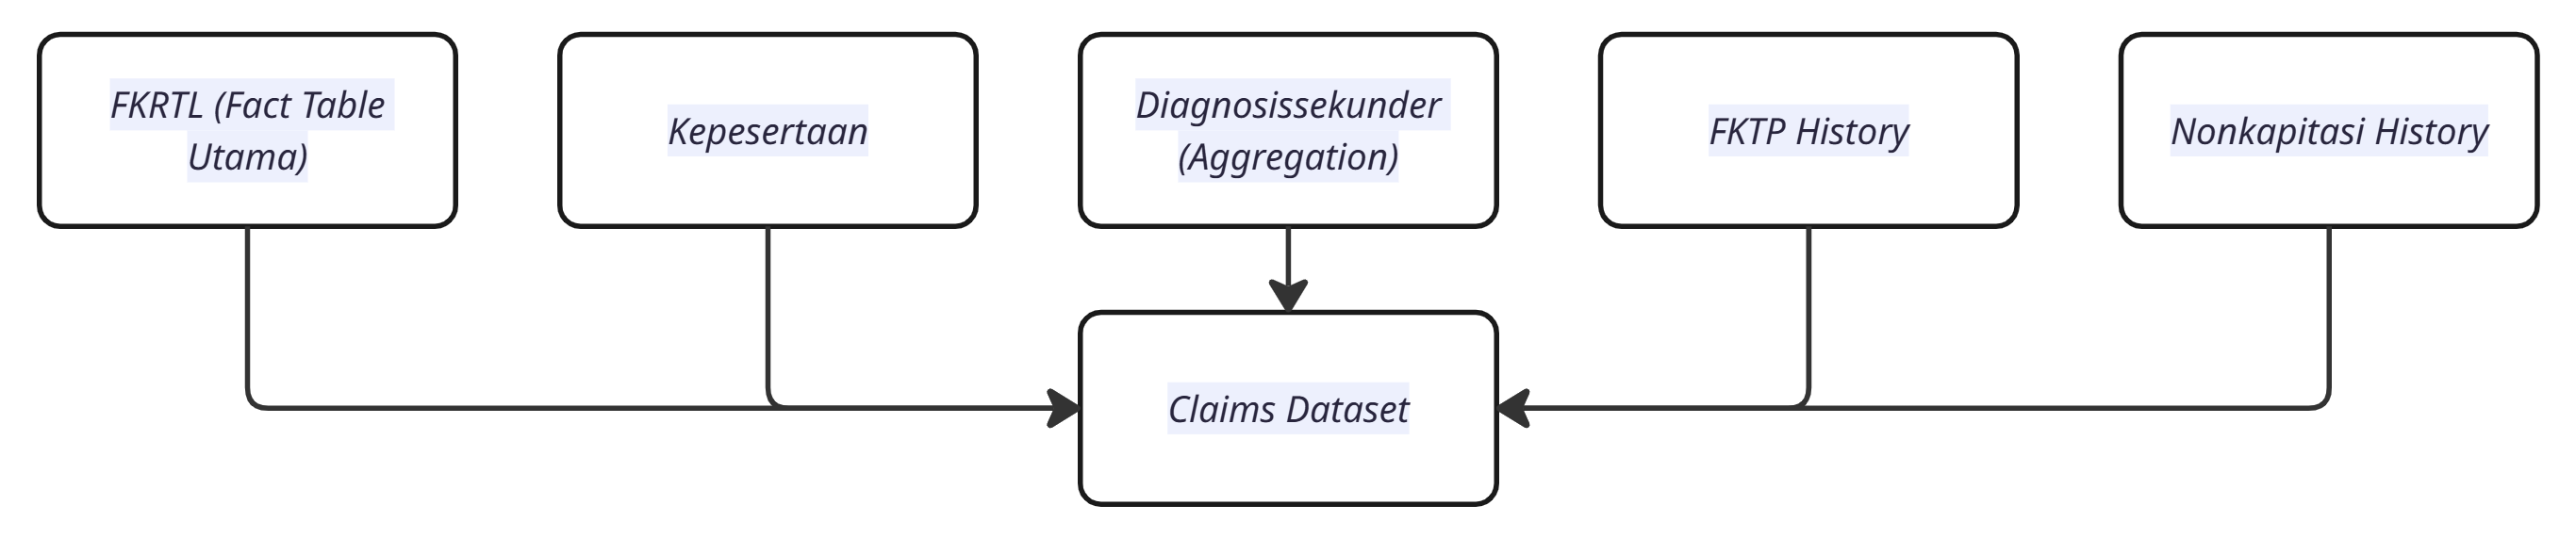
\includegraphics[width=5.51181in,height=1.15208in]{media/media/image10.png}

\phantomsection\label{_Toc228109338}{}Gambar 4. 1 Diagram Integrasi Claim-Centric

Berdasarkan Gambar 4.1, alur integrasi dimulai dari~FKRTL~sebagai pusat analisis, lalu diperkaya melalui integrasi atribut~kepesertaan, agregasi~diagnosissekunder, serta pembentukan histori layanan dari~FKTP~dan~nonkapitasi. Hasil akhir dari tahapan tersebut adalah terbentuknya~claims dataset, yaitu dataset analitis pada level klaim yang siap digunakan untuk proses pembersihan lanjutan, pembentukan fitur, dan pemodelan.

Untuk memperjelas sumber variabel yang masuk ke dalam proses integrasi, ringkasan asal data, variabel yang diambil, dan hasil integrasinya ditunjukkan pada Tabel 4.11.

\phantomsection\label{_Toc228109416}{}Tabel 4. 11 Ringkasan Integrasi Claim-Centric

\begin{longtable}[]{@{}
  >{\raggedright\arraybackslash}p{(\columnwidth - 4\tabcolsep) * \real{0.2510}}
  >{\raggedright\arraybackslash}p{(\columnwidth - 4\tabcolsep) * \real{0.4427}}
  >{\raggedright\arraybackslash}p{(\columnwidth - 4\tabcolsep) * \real{0.3063}}@{}}
\toprule\noalign{}
\begin{minipage}[b]{\linewidth}\raggedright
\textbf{Sumber}
\end{minipage} & \begin{minipage}[b]{\linewidth}\raggedright
\textbf{Variabel yang Diambil}
\end{minipage} & \begin{minipage}[b]{\linewidth}\raggedright
\textbf{Hasil Integrasi}
\end{minipage} \\
\midrule\noalign{}
\endhead
\bottomrule\noalign{}
\endlastfoot
fkrtl & id\_klaim,~id\_peserta, tanggal layanan, tarif, severity, atribut klaim utama & Menjadi struktur dasar dataset klaim \\
kepesertaan & jenis kelamin, tanggal lahir, status kepesertaan, atribut peserta & Menambah konteks peserta pada klaim \\
diagnosissekunder & kode diagnosis sekunder, grup diagnosis sekunder & Membentuk agregasi diagnosis sekunder per klaim \\
fktpkapitasi & tanggal pelayanan dan riwayat kunjungan FKTP & Membentuk fitur histori layanan FKTP \\
nonkapitasi & tanggal pelayanan dan biaya layanan nonkapitasi & Membentuk fitur histori layanan dan biaya nonkapitasi \\
\end{longtable}

Tabel 4.11 memperlihatkan bahwa setiap sumber data menyumbang informasi yang berbeda ke dalam struktur akhir klaim.~fkrtl~menyumbang identitas klaim dan komponen inti pelayanan,~kepesertaan~menyumbang atribut peserta,~diagnosissekunder~menyumbang ringkasan diagnosis tambahan, sedangkan~fktpkapitasi~dan~nonkapitasi~menyumbang histori layanan peserta sebelum klaim terjadi. Dengan susunan seperti ini, dataset hasil integrasi tidak hanya kaya secara informasi, tetapi juga tetap konsisten karena seluruh pengayaan dilakukan di sekitar unit analisis yang sama, yaitu klaim.

\subsection{Karakteristik Variabel dan Feature Engineering}\label{karakteristik-variabel-dan-feature-engineering}

Setelah integrasi data selesai dilakukan, tahapan berikutnya adalah pembentukan fitur yang digunakan untuk eksperimen. Fitur-fitur pada penelitian ini tidak dibangun secara acak, tetapi disusun ke dalam beberapa kelompok besar berdasarkan fungsi analitisnya, yaitu fitur demografis, biaya, klinis, diagnosis, histori layanan, dan rasio turunan. Pengelompokan ini penting karena setiap kelompok fitur mewakili dimensi yang berbeda dalam membaca karakteristik klaim.

Fitur demografis digunakan untuk merepresentasikan profil dasar peserta, seperti usia dan jenis kelamin. Fitur biaya digunakan untuk menangkap besaran finansial klaim, baik dalam bentuk nilai absolut maupun biaya turunan. Fitur klinis digunakan untuk menggambarkan tingkat keparahan pelayanan dan karakteristik perawatan. Sementara itu, fitur diagnosis digunakan untuk menangkap intensitas diagnosis sekunder, fitur histori layanan digunakan untuk merekam pola utilisasi sebelum klaim, dan rasio turunan digunakan untuk menyoroti ketidakwajaran relatif antar komponen biaya dan histori layanan.

Untuk memberikan gambaran awal mengenai karakteristik dataset, penelitian ini menampilkan distribusi empat variabel numerik utama, yaitu~usia,~lama\_rawat\_hari,~severity\_level, dan~tarif\_disetujui. Keempat variabel tersebut dipilih karena mewakili dimensi penting dalam data klaim, yaitu profil peserta, karakteristik pelayanan klinis, tingkat keparahan kasus, dan besaran finansial klaim.

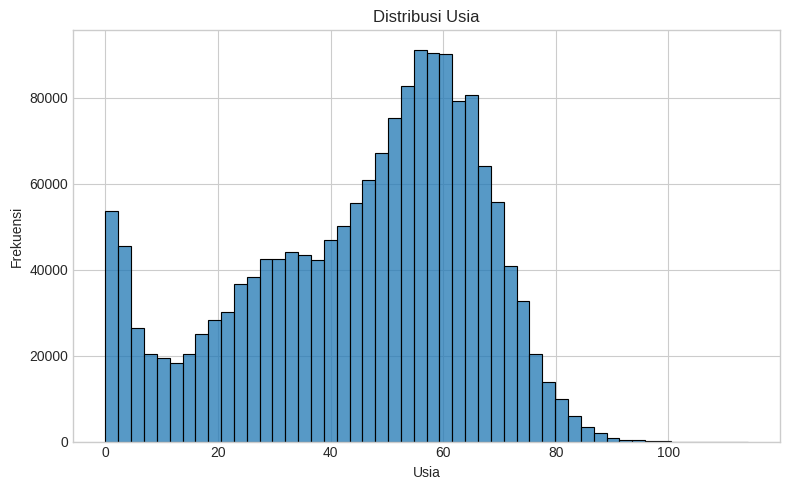
\includegraphics[width=5.51181in,height=3.41736in]{media/media/image11.png}

\phantomsection\label{_Toc228109339}{}Gambar 4. 2 Distribusi Usia

Distribusi~usia~ditunjukkan pada~Gambar 4.2. Gambar tersebut memperlihatkan bahwa data mencakup rentang usia yang luas, sehingga profil peserta pada dataset tidak terkonsentrasi hanya pada satu kelompok umur tertentu. Sebaran ini menunjukkan bahwa model perlu menangani variasi karakteristik peserta yang cukup beragam pada level klaim.

Distribusi~lama\_rawat\_hari~ditunjukkan pada~Gambar 4.3. Berdasarkan gambar tersebut, durasi rawat cenderung terkonsentrasi pada nilai yang lebih rendah, namun tetap memiliki ekor distribusi yang panjang. Pola ini menunjukkan bahwa sebagian besar klaim berkaitan dengan lama rawat yang singkat, sementara sebagian lainnya memiliki durasi yang jauh lebih panjang dan berpotensi memberikan sinyal klinis maupun finansial yang berbeda.

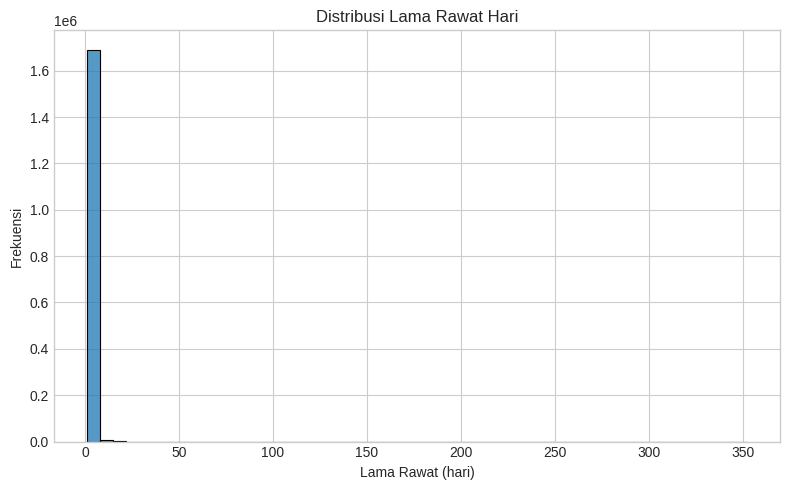
\includegraphics[width=5.51181in,height=3.41736in]{media/media/image12.png}

\phantomsection\label{_Toc228109340}{}Gambar 4. 3 Distribusi Lama Rawat Hari

Distribusi~severity\_level~ditunjukkan pada~Gambar 4.4. Variabel ini penting karena merepresentasikan tingkat keparahan kasus pada klaim. Sebaran pada gambar tersebut menunjukkan bahwa tingkat keparahan tidak homogen, sehingga model perlu mempertimbangkan variasi kompleksitas kasus sebagai salah satu unsur penting dalam membaca kewajaran klaim.

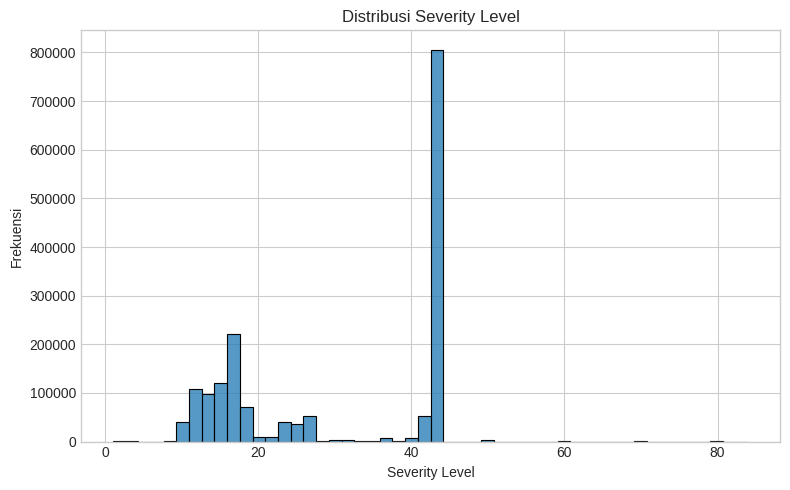
\includegraphics[width=5.51181in,height=3.41736in]{media/media/image13.png}

\phantomsection\label{_Toc228109341}{}Gambar 4. 4 Distribusi Severity Level

Distribusi~tarif\_disetujui~ditunjukkan pada~Gambar 4.5. Gambar tersebut memperlihatkan bahwa nilai biaya klaim memiliki rentang yang sangat lebar, dengan sebagian klaim berada pada kisaran biaya yang jauh lebih tinggi daripada Meioritas populasi. Variasi finansial yang besar ini menunjukkan bahwa komponen biaya memiliki posisi penting dalam eksperimen, terutama pada tahap pseudo-labeling dan seleksi fitur, karena pola anomali biaya berpotensi menjadi salah satu penanda utama klaim berisiko.

Secara keseluruhan, keempat distribusi tersebut menunjukkan bahwa dataset pada penelitian ini memiliki keragaman yang cukup besar dari sisi peserta, pelayanan, keparahan klinis, dan nilai finansial. Karakteristik inilah yang kemudian menjadi dasar penting dalam pembentukan pseudo-label, preprocessing, dan pemilihan konfigurasi fitur pada tahap pemodelan.

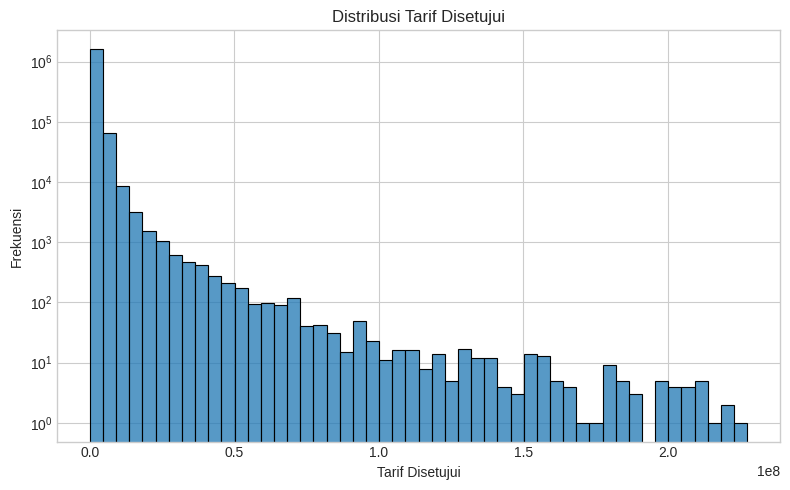
\includegraphics[width=5.51181in,height=3.41736in]{media/media/image14.png}

\phantomsection\label{_Toc228109342}{}Gambar 4. 5 Distribusi Tarif Disetujui

Untuk memperjelas susunan kelompok fitur yang digunakan pada dataset akhir, ringkasan kelompok fitur beserta contoh variabel dan tujuan analitisnya disajikan pada Tabel 4.12.

\phantomsection\label{_Toc228109417}{}Tabel 4. 12 Kelompok Fitur Final

\begin{longtable}[]{@{}
  >{\raggedright\arraybackslash}p{(\columnwidth - 4\tabcolsep) * \real{0.2498}}
  >{\raggedright\arraybackslash}p{(\columnwidth - 4\tabcolsep) * \real{0.4168}}
  >{\raggedright\arraybackslash}p{(\columnwidth - 4\tabcolsep) * \real{0.3334}}@{}}
\toprule\noalign{}
\begin{minipage}[b]{\linewidth}\raggedright
\textbf{Kelompok Fitur}
\end{minipage} & \begin{minipage}[b]{\linewidth}\raggedright
\textbf{Contoh Variabel}
\end{minipage} & \begin{minipage}[b]{\linewidth}\raggedright
\textbf{Tujuan Analitis}
\end{minipage} \\
\midrule\noalign{}
\endhead
\bottomrule\noalign{}
\endlastfoot
Demografis & usia,~gender\_singkat & Menggambarkan profil dasar peserta \\
Biaya & tarif\_disetujui,~tarif\_inacbg\_dasar,~biaya\_per\_hari & Menangkap pola finansial klaim \\
Klinis & severity\_level,~lama\_rawat\_hari,~total\_special\_cmg & Menggambarkan tingkat keparahan dan karakteristik layanan \\
Diagnosis & jumlah\_diagnosis\_sekunder,~jumlah\_grup\_diagnosis\_sekunder & Mengukur intensitas diagnosis tambahan \\
Histori layanan & fktp\_hist\_count\_before,~nonkap\_hist\_count\_before & Menangkap pola utilisasi sebelum klaim \\
Rasio turunan & rasio\_tarif\_setuju\_vs\_dasar,~rasio\_biaya\_klaim\_vs\_histori\_nonkap & Menyoroti hubungan relatif antar komponen biaya dan histori \\
\end{longtable}

Tabel 4.12 menunjukkan bahwa setiap kelompok fitur memiliki peran analitis yang berbeda. Fitur demografis membantu membaca konteks peserta, fitur biaya menggambarkan beban finansial klaim, fitur klinis memperlihatkan tingkat keparahan dan karakteristik pelayanan, fitur diagnosis menangkap intensitas kondisi tambahan, fitur histori layanan memberikan konteks utilisasi sebelum klaim, dan rasio turunan membantu menilai hubungan relatif antar komponen biaya dan riwayat layanan. Dengan pengelompokan tersebut, dataset akhir pada penelitian ini tidak hanya kaya secara jumlah fitur, tetapi juga kaya secara makna analitis.

\subsection{Implikasi Karakteristik Data terhadap Eksperimen}\label{implikasi-karakteristik-data-terhadap-eksperimen}

Karakteristik data yang telah dijelaskan pada subbab sebelumnya memiliki implikasi langsung terhadap pembentukan model. Salah satu implikasi utama adalah munculnya ketidakseimbangan label setelah tahap pseudo-labeling. Karena klaim yang ditandai sebagai anomali hanya merupakan sebagian kecil dari keseluruhan populasi, maka model harus dibangun pada kondisi distribusi kelas yang tidak seimbang. Kondisi ini berpengaruh pada pemilihan metrik evaluasi, teknik preprocessing, serta kebutuhan~\emph{threshold tuning}~pada tahap akhir.

Implikasi berikutnya adalah besarnya variasi nilai biaya antar klaim. Variabel seperti~tarif\_disetujui~dan komponen biaya lainnya menunjukkan rentang yang sangat lebar, sehingga tanpa preprocessing yang tepat, model dapat terdorong terlalu kuat oleh variabel biaya mentah. Oleh karena itu, transformasi numerik, pembentukan rasio turunan, dan mekanisme seleksi fitur menjadi penting agar model tidak hanya sensitif terhadap besaran biaya absolut, tetapi juga terhadap pola ketidakwajaran yang lebih informatif.

Karakteristik data juga menunjukkan bahwa histori layanan memiliki posisi penting dalam eksperimen. Kehadiran fitur histori dari~fktpkapitasi~dan~nonkapitasi~memungkinkan model tidak hanya membaca klaim sebagai transaksi tunggal, tetapi juga sebagai bagian dari riwayat pemanfaatan layanan peserta. Dengan adanya konteks historis tersebut, model memiliki dasar yang lebih kuat untuk membedakan klaim yang memang tinggi karena pola pelayanan sebelumnya dengan klaim yang tampak menyimpang secara tidak wajar.

Selain itu, kompleksitas struktur data yang terbentuk dari integrasi multi-tabel membuat tahap preprocessing dan~\emph{feature selection}~menjadi keharusan, bukan pelengkap. Banyaknya fitur dengan tipe yang berbeda, kemungkinan redundansi antarvariabel, serta potensi multikolinearitas menjadikan proses seleksi fitur sebagai bagian penting dalam eksperimen. Dengan kata lain, karakteristik data pada penelitian ini secara langsung menjelaskan mengapa eksperimen memerlukan tahapan split yang terkontrol, preprocessing yang sistematis, dan beberapa~\emph{branch feature selection}~sebelum masuk ke tahap benchmarking model.

Secara keseluruhan, karakteristik data pada penelitian ini membentuk dasar teknis bagi seluruh eksperimen yang dilakukan. Struktur data yang kaya, skala data yang besar, variasi biaya yang tinggi, serta distribusi label yang tidak seimbang menjadikan eksperimen tidak dapat dilakukan dengan pendekatan klasifikasi sederhana. Justru karena karakteristik data itulah, pipeline final pada penelitian ini dirancang dalam bentuk integrasi berbasis klaim, pseudo-labeling, seleksi fitur bertingkat, benchmarking multi-model, dan evaluasi yang dilengkapi interpretabilitas.

\section{TEMPAT UJI COBA}\label{tempat-uji-coba}

Subbab ini menjelaskan lingkungan tempat eksperimen dijalankan. Penjelasan mengenai tempat ujicoba diperlukan agar pelaksanaan eksperimen dapat dipahami dalam konteks lingkungan komputasi yang digunakan, termasuk platform notebook, ruang kerja eksekusi, dan lokasi penyimpanan artefak hasil. Dengan mencantumkan lingkungan ujicoba secara jelas, hasil eksperimen pada penelitian ini dapat dibaca sebagai keluaran dari proses yang dijalankan pada satu lingkungan komputasi yang konsisten.

Eksperimen pada penelitian ini dijalankan pada platform komputasi berbasis notebook dengan lingkungan kerja Python yang mendukung proses pengolahan data, pemodelan, evaluasi, dan interpretabilitas. Lingkungan tersebut memungkinkan seluruh pipeline dijalankan secara terintegrasi, mulai dari pembacaan tabel mentah, pembentukan dataset berbasis klaim, pelaksanaan benchmarking model, hingga penyimpanan artefak hasil eksperimen. Dengan demikian, tempat ujicoba pada penelitian ini tidak dipahami sebagai lokasi fisik semata, tetapi sebagai lingkungan komputasi tempat seluruh eksperimen dijalankan.

Lingkungan notebook yang digunakan juga berperan sebagai ruang kerja utama selama eksperimen berlangsung. Seluruh tahapan analisis dilakukan di dalam notebook yang sama, sehingga alur eksperimen dapat dijalankan secara runtut dan terdokumentasi dengan baik. Hal ini penting karena pipeline penelitian ini tidak terdiri atas satu tahap tunggal, melainkan serangkaian proses yang saling terkait dari awal sampai akhir.

Selain sebagai tempat eksekusi, lingkungan ujicoba pada penelitian ini juga menjadi lokasi keluaran artefak eksperimen. Artefak seperti informasi model pemenang, analisis threshold, hasil evaluasi akhir, dan keluaran interpretabilitas disimpan pada direktori kerja notebook, sehingga dapat digunakan kembali untuk kebutuhan pelaporan dan analisis lanjutan. Ringkasan komponen lingkungan ujicoba yang digunakan pada penelitian ini ditunjukkan pada Tabel 4.13.

\phantomsection\label{_Toc228109418}{}Tabel 4. 13 Lingkungan Uji Coba

\begin{longtable}[]{@{}
  >{\raggedright\arraybackslash}p{(\columnwidth - 2\tabcolsep) * \real{0.2538}}
  >{\raggedright\arraybackslash}p{(\columnwidth - 2\tabcolsep) * \real{0.7462}}@{}}
\toprule\noalign{}
\begin{minipage}[b]{\linewidth}\raggedright
\textbf{Komponen}
\end{minipage} & \begin{minipage}[b]{\linewidth}\raggedright
\textbf{Deskripsi}
\end{minipage} \\
\midrule\noalign{}
\endhead
\bottomrule\noalign{}
\endlastfoot
Platform komputasi & Lingkungan komputasi berbasis notebook cloud \\
Lingkungan notebook & Notebook Python yang digunakan untuk menjalankan seluruh pipeline eksperimen \\
Lokasi output artefak & Hasil pekerjaan disimpan dalam bentul Notebook .ipynb di platform Kaggle \\
\end{longtable}

Berdasarkan Tabel 4.13, lingkungan ujicoba pada penelitian ini terdiri atas tiga komponen utama, yaitu platform komputasi, lingkungan notebook, dan lokasi penyimpanan artefak hasil. Platform komputasi berfungsi sebagai tempat pelaksanaan seluruh eksperimen, lingkungan notebook berfungsi sebagai ruang kerja interaktif untuk menjalankan pipeline, sedangkan direktori keluaran artefak menjadi lokasi penyimpanan hasil eksperimen yang dihasilkan selama proses analisis. Dengan susunan tersebut, eksperimen pada penelitian ini dijalankan dalam lingkungan yang terpusat dan konsisten, sehingga seluruh keluaran dapat ditelusuri kembali dengan lebih mudah.

\section{WAKTU UJI COBA}\label{waktu-uji-coba}

Subbab ini menjelaskan waktu pelaksanaan eksperimen dan rerun final yang dijadikan dasar hasil pada Bab 4. Penjelasan waktu ujicoba penting untuk menegaskan bahwa hasil yang dibahas pada bab ini tidak diambil secara acak dari beberapa versi eksperimen yang berbeda, melainkan berasal dari satu pelaksanaan final yang dijadikan acuan utama.

Pelaksanaan eksperimen pada penelitian ini berlangsung pada tahap pengolahan data, pemodelan, evaluasi, dan interpretabilitas dalam lingkungan notebook final. Dari keseluruhan proses tersebut, hasil yang digunakan sebagai dasar penulisan Bab 4 diturunkan dari rerun final notebook yang menghasilkan keluaran eksperimen lengkap dan artefak hasil yang konsisten. Penetapan rerun final sebagai acuan utama diperlukan agar semua angka, tabel, dan pembahasan pada bab ini berasal dari satu konfigurasi eksperimen yang sama.

Waktu rerun final menjadi penanda penting karena menunjukkan titik ketika pipeline telah dijalankan dengan konfigurasi akhir yang stabil. Dengan demikian, hasil pada Bab 4 merepresentasikan kondisi akhir eksperimen yang digunakan dalam penelitian ini, bukan keluaran antara atau percobaan awal yang belum final. Ringkasan tahapan waktu pelaksanaan ujicoba dan rerun final yang digunakan sebagai dasar hasil Bab 4 ditunjukkan pada Tabel 4.14.

\phantomsection\label{_Toc228109419}{}Tabel 4. 14 Waktu Pelaksanaan Uji Coba

\begin{longtable}[]{@{}
  >{\raggedright\arraybackslash}p{(\columnwidth - 4\tabcolsep) * \real{0.2378}}
  >{\raggedright\arraybackslash}p{(\columnwidth - 4\tabcolsep) * \real{0.4049}}
  >{\raggedright\arraybackslash}p{(\columnwidth - 4\tabcolsep) * \real{0.3573}}@{}}
\toprule\noalign{}
\begin{minipage}[b]{\linewidth}\raggedright
\textbf{Tahap}
\end{minipage} & \begin{minipage}[b]{\linewidth}\raggedright
\textbf{Waktu Pelaksanaan}
\end{minipage} & \begin{minipage}[b]{\linewidth}\raggedright
\textbf{Keterangan}
\end{minipage} \\
\midrule\noalign{}
\endhead
\bottomrule\noalign{}
\endlastfoot
Persiapan eksperimen & Periode pengolahan data dan penyusunan pipeline & Mencakup integrasi data dan rekayasa fitur \\
Pelaksanaan eksperimen & Periode benchmarking, evaluasi, dan interpretabilitas & Mencakup seluruh tahapan pengujian model \\
Rerun final notebook & 17 April 2026 & Menjadi dasar hasil yang digunakan pada Bab 4 \\
\end{longtable}

Tabel 4.14 menunjukkan bahwa pelaksanaan eksperimen pada penelitian ini dapat dibedakan ke dalam tahap persiapan eksperimen, pelaksanaan pipeline, dan rerun final yang dijadikan dasar penulisan hasil. Keberadaan kolom keterangan pada tabel tersebut penting karena memberikan konteks terhadap masing-masing tahap, terutama untuk menegaskan bahwa pembahasan pada Bab 4 diturunkan dari rerun final, bukan dari hasil uji coba sementara. Dengan demikian, pembaca dapat memahami bahwa hasil yang dibahas pada bab ini memiliki titik acuan waktu yang jelas dan konsisten.

\section{SPESIFIKASI PERALATAN UJI COBA}\label{spesifikasi-peralatan-uji-coba}

Subbab ini menjelaskan perangkat keras, perangkat lunak, dan pustaka utama yang digunakan selama eksperimen. Penjelasan ini diperlukan agar pembaca memperoleh gambaran yang jelas mengenai perangkat dan lingkungan teknis yang mendukung pelaksanaan pipeline penelitian, mulai dari pengolahan data sampai interpretabilitas model.

Eksperimen pada penelitian ini dijalankan pada lingkungan notebook komputasi berbasis Python. Karena pelaksanaan eksperimen dilakukan pada platform notebook, maka spesifikasi peralatan pada penelitian ini dijelaskan dalam bentuk lingkungan komputasi yang digunakan, bahasa pemrograman, serta pustaka-pustaka utama yang benar-benar dipakai dalam pipeline. Dengan pendekatan tersebut, penjelasan spesifikasi peralatan tetap relevan terhadap proses eksperimen yang dijalankan.

Dari sisi perangkat lunak, bahasa pemrograman utama yang digunakan adalah Python dengan lingkungan notebook interaktif. Lingkungan ini mendukung proses pembacaan data, transformasi, pembentukan fitur, pelatihan model, evaluasi metrik, visualisasi, dan interpretabilitas hasil. Struktur seperti ini membuat seluruh tahapan penelitian dapat dijalankan dalam satu lingkungan kerja yang terintegrasi.

Dari sisi pustaka, eksperimen ini memanfaatkan beberapa kelompok library utama. Library pengolahan data digunakan untuk membaca, membersihkan, dan mentransformasikan data tabular. Library pemodelan digunakan untuk menjalankan pseudo-labeling, preprocessing, benchmarking model, dan evaluasi performa. Sementara itu, library interpretabilitas digunakan untuk menjelaskan keluaran model pada tingkat global maupun lokal. Ringkasan spesifikasi peralatan ujicoba yang digunakan pada penelitian ini ditunjukkan pada Tabel 4.15.

\phantomsection\label{_Toc228109420}{}Tabel 4. 15 Spesifikasi Peralatan Uji Coba

\begin{longtable}[]{@{}
  >{\raggedright\arraybackslash}p{(\columnwidth - 4\tabcolsep) * \real{0.2498}}
  >{\raggedright\arraybackslash}p{(\columnwidth - 4\tabcolsep) * \real{0.3218}}
  >{\raggedright\arraybackslash}p{(\columnwidth - 4\tabcolsep) * \real{0.4284}}@{}}
\toprule\noalign{}
\begin{minipage}[b]{\linewidth}\raggedright
\textbf{Komponen}
\end{minipage} & \begin{minipage}[b]{\linewidth}\raggedright
\textbf{Spesifikasi}
\end{minipage} & \begin{minipage}[b]{\linewidth}\raggedright
\textbf{Fungsi}
\end{minipage} \\
\midrule\noalign{}
\endhead
\bottomrule\noalign{}
\endlastfoot
Perangkat komputasi & Lingkungan notebook cloud & Menjalankan seluruh proses eksperimen \\
Bahasa pemrograman & Python & Bahasa utama untuk pengolahan data dan pemodelan \\
Lingkungan kerja & Jupyter Notebook / Kaggle Notebook & Menjalankan pipeline secara interaktif \\
Library pengolahan data & pandas,~numpy & Membaca, membersihkan, dan mentransformasikan data \\
Library visualisasi & matplotlib,~seaborn & Membuat grafik dan visualisasi eksperimen \\
Library pemodelan & scikit-learn,~xgboost,~lightgbm,~catboost & Menjalankan pseudo-labeling, preprocessing, benchmarking, dan evaluasi \\
Library interpretabilitas & shap,~lime & Menjelaskan hasil prediksi model \\
Library tambahan & optuna~atau library tuning lain jika dipakai & Mendukung optimasi parameter model \\
\end{longtable}

Berdasarkan Tabel 4.15, spesifikasi peralatan ujicoba pada penelitian ini dapat dibaca sebagai kombinasi antara lingkungan komputasi notebook, bahasa pemrograman Python, serta pustaka-pustaka utama yang mendukung setiap tahap eksperimen. Komponen untuk pengolahan data berfungsi membentuk dataset analitis yang siap dipakai, komponen pemodelan berfungsi menjalankan pseudo-labeling dan benchmarking model, sedangkan komponen interpretabilitas berfungsi membaca dan menjelaskan keputusan model. Dengan konfigurasi seperti ini, seluruh tahapan eksperimen dapat dilaksanakan secara terpadu dalam satu lingkungan kerja yang konsisten.

\section{HASIL EKSPERIMEN}\label{hasil-eksperimen}

Subbab ini menyajikan hasil eksperimen yang diperoleh dari pelaksanaan pipeline final penelitian. Penyajian hasil dilakukan secara bertahap mengikuti urutan proses eksperimen, mulai dari pembentukan basis klaim, pembentukan dataset pemodelan, pseudo-labeling, pembagian data, seleksi fitur, benchmarking model, penetapan model final, evaluasi performa, interpretabilitas, hingga artefak hasil yang diekspor. Dengan susunan seperti ini, pembaca dapat mengikuti keluaran eksperimen secara runtut dari tahap awal hingga tahap akhir.

Berbeda dari pembahasan parameter eksperimen pada subbab sebelumnya, bagian ini berfokus pada keluaran aktual yang dihasilkan dari pipeline. Setiap subbagian pada 4.6 mewakili satu keluaran utama, sehingga hubungan antara tahapan eksperimen dan hasil yang diperoleh dapat dibaca dengan lebih jelas. Pendekatan ini juga memudahkan pembaca untuk melihat bagaimana satu tahap memengaruhi tahap berikutnya sampai akhirnya menghasilkan model final beserta interpretasinya.

\subsection{Hasil Integrasi Claim-Centric}\label{hasil-integrasi-claim-centric}

Tahap awal eksperimen menghasilkan pembentukan basis klaim melalui integrasi data berbasis~claim-centric. Pada tahap ini,~fkrtl~digunakan sebagai kerangka utama, kemudian diperkaya dengan atribut dari~kepesertaan, agregasi dari~diagnosissekunder, serta histori layanan dari~fktpkapitasi~dan~nonkapitasi. Hasil integrasi ini menjadi fondasi bagi seluruh eksperimen karena seluruh tahapan selanjutnya dijalankan di atas dataset klaim yang telah diperkaya.

Berdasarkan hasil integrasi, jumlah observasi akhir tetap berada pada level klaim dan tidak berubah menjadi level peserta atau level kunjungan. Hal ini menunjukkan bahwa strategi integrasi yang digunakan berhasil mempertahankan satu klaim sebagai satu unit observasi utama. Dengan demikian, struktur akhir dataset tetap selaras dengan tujuan penelitian, yaitu mendeteksi potensi fraud atau upcoding pada level transaksi klaim.

Ringkasan hasil integrasi~claim-centric~ditunjukkan pada Tabel 4.16. Tabel tersebut memperlihatkan tahapan utama pembentukan basis klaim, keluaran pada setiap tahap, serta ukuran data yang dihasilkan.

\phantomsection\label{_Toc228109421}{}Tabel 4. 16 Hasil Integrasi Claim-Centric

\begin{longtable}[]{@{}
  >{\raggedright\arraybackslash}p{(\columnwidth - 4\tabcolsep) * \real{0.3333}}
  >{\raggedright\arraybackslash}p{(\columnwidth - 4\tabcolsep) * \real{0.3333}}
  >{\raggedright\arraybackslash}p{(\columnwidth - 4\tabcolsep) * \real{0.3334}}@{}}
\toprule\noalign{}
\begin{minipage}[b]{\linewidth}\raggedright
\textbf{Tahap}
\end{minipage} & \begin{minipage}[b]{\linewidth}\raggedright
\textbf{Output}
\end{minipage} & \begin{minipage}[b]{\linewidth}\raggedright
\textbf{Ukuran Data}
\end{minipage} \\
\midrule\noalign{}
\endhead
\bottomrule\noalign{}
\endlastfoot
Pemuatan~fkrtl & Basis klaim awal & 1.699.219 x 57 \\
Integrasi dengan~kepesertaan & Klaim dengan atribut peserta & sesuai hasil merge \\
Agregasi~diagnosissekunder & Klaim dengan ringkasan diagnosis sekunder & sesuai hasil agregasi \\
Integrasi histori~fktpkapitasi~dan~nonkapitasi & Klaim dengan fitur histori layanan & sesuai hasil integrasi akhir \\
Pembentukan~claims & Dataset klaim final sebelum feature engineering & 1.699.219 x 79 \\
\end{longtable}

Berdasarkan Tabel 4.16, hasil integrasi menghasilkan struktur klaim akhir yang memuat informasi peserta, diagnosis sekunder, dan histori layanan dalam satu dataset yang tetap terpusat pada klaim. Hal ini penting karena kualitas tahap integrasi akan menentukan kualitas fitur yang dibentuk pada tahap berikutnya. Dengan kata lain, keberhasilan eksperimen pada tahap pemodelan sangat bergantung pada keberhasilan pembentukan basis klaim pada tahap ini.

\subsection{Hasil Feature Engineering dan Modeling Dataset}\label{hasil-feature-engineering-dan-modeling-dataset}

Setelah basis klaim terbentuk, eksperimen dilanjutkan ke tahap~\emph{feature engineering}~untuk membangun variabel yang digunakan pada pemodelan. Pada tahap ini, fitur akhir dibentuk dari kombinasi informasi administratif, klinis, biaya, diagnosis, serta histori layanan. Hasil pembentukan fitur tersebut kemudian dihimpun ke dalam~model\_df, yaitu dataset pemodelan yang menjadi dasar seluruh tahap eksperimen selanjutnya.

Hasil eksperimen menunjukkan bahwa model\_df berhasil dibentuk dengan ukuran yang besar dan mencakup fitur-fitur yang dibutuhkan untuk tahap unsupervised maupun supervised. Struktur ini penting karena model\_df menjadi titik pertemuan antara hasil integrasi data, rekayasa fitur, dan kebutuhan pemodelan, sehingga kualitas serta kelengkapan fitur pada tahap ini sangat menentukan kualitas pseudo-labeling dan proses benchmarking berikutnya.

Tabel 4.17 menunjukkan bahwa dataset pemodelan akhir terdiri atas 1.699.219 observasi dengan 51 kolom, 14 fitur unsupervised, dan seperangkat fitur supervised final yang digunakan pada tahap klasifikasi. Susunan ini menunjukkan bahwa hasil feature engineering tidak hanya memperkaya data klaim, tetapi juga menghasilkan struktur dataset yang siap dipakai secara langsung untuk membangun target awal, melatih model, dan mengevaluasi performa.

Untuk memperjelas hasil pembentukan dataset pemodelan, ringkasan komponen utama~model\_df~ditunjukkan pada Tabel 4.17.

\phantomsection\label{_Toc228109422}{}Tabel 4. 17 Ringkasan Modeling Dataset

\begin{longtable}[]{@{}
  >{\raggedright\arraybackslash}p{(\columnwidth - 2\tabcolsep) * \real{0.4997}}
  >{\raggedright\arraybackslash}p{(\columnwidth - 2\tabcolsep) * \real{0.5003}}@{}}
\toprule\noalign{}
\begin{minipage}[b]{\linewidth}\raggedright
\textbf{Komponen}
\end{minipage} & \begin{minipage}[b]{\linewidth}\raggedright
\textbf{Nilai}
\end{minipage} \\
\midrule\noalign{}
\endhead
\bottomrule\noalign{}
\endlastfoot
Jumlah observasi & 1.699.219 \\
Jumlah kolom~model\_df & 51 \\
Jumlah fitur unsupervised & 14 \\
Jumlah fitur supervised & sesuai daftar final \\
Unit analisis & Satu klaim \\
\end{longtable}

Tabel 4.17 menunjukkan ukuran dataset pemodelan, jumlah fitur yang dihimpun, serta peran~model\_df~sebagai dasar bagi tahap pseudo-labeling dan supervised learning. Dengan tersusunnya~model\_df, eksperimen pada penelitian ini memasuki tahap pemodelan dengan satu dataset akhir yang telah siap dipakai secara langsung.

Dengan terbentuknya model\_df, eksperimen pada penelitian ini memasuki tahap pemodelan dengan satu dataset akhir yang telah terintegrasi, bersih, dan relevan secara analitis. Oleh karena itu, hasil pada subbab ini menegaskan bahwa tahap feature engineering berhasil mengubah data klaim multi-sumber menjadi dataset pemodelan yang operasional untuk seluruh pipeline penelitian.

\subsection{Hasil Pseudo-Labeling dengan Isolation Forest}\label{hasil-pseudo-labeling-dengan-isolation-forest}

Setelah dataset pemodelan terbentuk, eksperimen dilanjutkan ke tahap pseudo-labeling menggunakan~Isolation Forest. Tahap ini dilakukan untuk membentuk target awal pada data yang semula tidak memiliki label fraud aktual. Pseudo-labeling menjadi penting karena tanpa target awal, eksperimen tidak dapat dilanjutkan ke tahap supervised benchmarking.

Hasil sensitivity analysis terhadap beberapa nilai~contamination rate~menunjukkan bahwa jumlah klaim yang ditandai sebagai anomali berubah secara proporsional terhadap nilai kontaminasi yang diuji. Pada tingkat~0,01, jumlah klaim anomali berada pada kisaran terendah, sedangkan pada tingkat~0,10, jumlah klaim anomali meningkat jauh lebih besar. Variasi ini menunjukkan bahwa hasil pseudo-labeling sensitif terhadap asumsi proporsi anomali, sehingga pemilihan konfigurasi final perlu dilakukan secara hati-hati.

Hasil pseudo-labeling pada konfigurasi final menunjukkan bahwa jumlah klaim yang diberi label berisiko berada pada proporsi kecil dibandingkan total populasi klaim. Kondisi ini memperlihatkan bahwa pseudo-label yang terbentuk memang merepresentasikan anomali sebagai kelompok minoritas, sesuai dengan karakter umum fraud detection. Ringkasan hasil sensitivity pseudo-labeling ditunjukkan pada Tabel 4.18.

\phantomsection\label{_Toc228109423}{}Tabel 4. 18 Sensitivity Pseudo-Labeling

\begin{longtable}[]{@{}
  >{\raggedright\arraybackslash}p{(\columnwidth - 6\tabcolsep) * \real{0.3211}}
  >{\raggedright\arraybackslash}p{(\columnwidth - 6\tabcolsep) * \real{0.2680}}
  >{\raggedright\arraybackslash}p{(\columnwidth - 6\tabcolsep) * \real{0.1608}}
  >{\raggedright\arraybackslash}p{(\columnwidth - 6\tabcolsep) * \real{0.2501}}@{}}
\toprule\noalign{}
\begin{minipage}[b]{\linewidth}\raggedright
\textbf{Contamination Rate}
\end{minipage} & \begin{minipage}[b]{\linewidth}\raggedright
\textbf{Jumlah Anomali}
\end{minipage} & \begin{minipage}[b]{\linewidth}\raggedright
\textbf{Rasio}
\end{minipage} & \begin{minipage}[b]{\linewidth}\raggedright
\textbf{Median Score}
\end{minipage} \\
\midrule\noalign{}
\endhead
\bottomrule\noalign{}
\endlastfoot
0,01 & 16.993 & 0,01 & 0,370421 \\
0,03 & 50.977 & 0,03 & 0,370421 \\
0,05 & 84.961 & 0,05 & 0,370421 \\
0,10 & 169.922 & 0,10 & 0,370421 \\
\end{longtable}

Berdasarkan Tabel 4.18, nilai~contamination rate~sebesar~0,03~menghasilkan sekitar~50.977~klaim anomali dengan rasio sekitar~3\%~dari total populasi. Hasil ini memperlihatkan bahwa distribusi label akhir bersifat tidak seimbang, dengan Meioritas klaim berada pada kelas normal. Kondisi tersebut menjadi salah satu karakter utama data yang akan memengaruhi pemilihan metrik evaluasi dan perlunya threshold tuning pada tahap berikutnya.

Selain jumlah anomali, eksperimen ini juga membandingkan profil median antara klaim normal dan klaim yang diberi pseudo-label berisiko. Perbandingan tersebut memberikan gambaran awal mengenai karakteristik yang membedakan kedua kelompok. Profil median pseudo-label ditunjukkan pada Gambar 4.6.

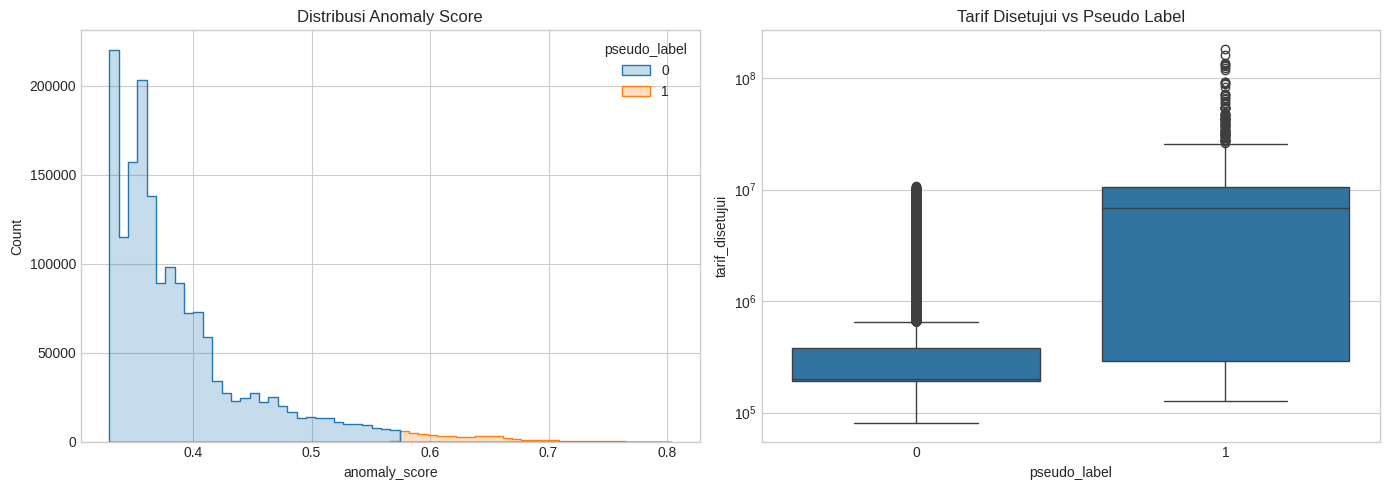
\includegraphics[width=5.51181in,height=1.94306in]{media/media/image15.png}

\phantomsection\label{_Toc228109343}{}Gambar 4. 6 Profil Median Pseudo-Label

Berdasarkan Gambar 4.6, klaim yang masuk ke kelompok~suspicious~cenderung memiliki nilai median yang lebih tinggi pada variabel biaya dan beberapa indikator layanan dibandingkan kelompok~normal. Perbedaan median ini menunjukkan bahwa pseudo-label yang terbentuk bukan bersifat acak, melainkan memiliki pola yang cukup jelas dalam membedakan klaim menyimpang dan klaim normal.

\subsection{Hasil Train/Validation/Test Split dan Preprocessing}\label{hasil-trainvalidationtest-split-dan-preprocessing}

Setelah pseudo-label dibentuk, dataset dibagi ke dalam tiga subset utama, yaitu~train,~validation, dan~test. Hasil pembagian data menunjukkan bahwa ukuran masing-masing subset sesuai dengan konfigurasi eksperimen dan distribusi label tetap terjaga secara konsisten antar subset. Hal ini penting untuk memastikan bahwa proses pelatihan, validasi, dan evaluasi berlangsung pada distribusi kelas yang sebanding.

Hasil eksperimen menunjukkan bahwa~train set~berisi~1.019.531~observasi, sedangkan~validation set~dan~test set~masing-masing berisi~339.844~observasi. Rasio pseudo-label positif pada ketiga subset tetap berada di sekitar~3\%, sehingga pembagian data dapat dikatakan berhasil mempertahankan komposisi kelas. Ringkasan hasil split dataset ditunjukkan pada Tabel 4.19.

\phantomsection\label{_Toc228109424}{}Tabel 4. 19 Hasil Split Dataset

\begin{longtable}[]{@{}
  >{\raggedright\arraybackslash}p{(\columnwidth - 4\tabcolsep) * \real{0.3333}}
  >{\raggedright\arraybackslash}p{(\columnwidth - 4\tabcolsep) * \real{0.3333}}
  >{\raggedright\arraybackslash}p{(\columnwidth - 4\tabcolsep) * \real{0.3333}}@{}}
\toprule\noalign{}
\begin{minipage}[b]{\linewidth}\raggedright
\textbf{Subset}
\end{minipage} & \begin{minipage}[b]{\linewidth}\raggedright
\textbf{Jumlah Data}
\end{minipage} & \begin{minipage}[b]{\linewidth}\raggedright
\textbf{Fraud Ratio}
\end{minipage} \\
\midrule\noalign{}
\endhead
\bottomrule\noalign{}
\endlastfoot
Train & 1.019.531 & 0,030000 \\
Validation & 339.844 & 0,030002 \\
Test & 339.844 & 0,029999 \\
\end{longtable}

Berdasarkan Tabel 4.19, konsistensi~fraud ratio~pada ketiga subset memperlihatkan bahwa proses split berjalan dengan baik dan tidak menimbulkan distorsi distribusi label. Hasil ini penting karena kestabilan distribusi kelas antar subset akan memengaruhi kualitas evaluasi model. Selain itu, tahap preprocessing yang dilakukan setelah split memastikan bahwa fitur numerik dan kategorikal dapat digunakan secara konsisten oleh seluruh model pada tahap benchmarking.

\subsection{Hasil Branch-Based Feature Selection}\label{hasil-branch-based-feature-selection}

Tahap berikutnya pada eksperimen adalah~branch-based feature selection. Pada tahap ini, beberapa strategi seleksi fitur dibandingkan untuk melihat bagaimana variasi himpunan fitur memengaruhi performa model. Eksperimen ini menghasilkan lima branch utama, yaitu domain\_expert, correlation, vif, permutation, dan~combined.

Hasil seleksi menunjukkan bahwa setiap branch menghasilkan jumlah fitur yang berbeda.~domain\_expert~menghasilkan himpunan fitur yang lebih ringkas, sedangkan~vif~menghasilkan jumlah fitur yang lebih besar dibandingkan branch lainnya.~permutation~dan~combined~menghasilkan struktur fitur yang berbeda lagi, sehingga eksperimen memiliki beberapa alternatif konfigurasi input sebelum masuk ke tahap benchmarking model.

Ringkasan hasil branch feature selection ditunjukkan pada Tabel 4.20.

\phantomsection\label{_Toc228109425}{}Tabel 4. 20 Ringkasan Branch Feature Selection

\begin{longtable}[]{@{}
  >{\raggedright\arraybackslash}p{(\columnwidth - 6\tabcolsep) * \real{0.2140}}
  >{\raggedright\arraybackslash}p{(\columnwidth - 6\tabcolsep) * \real{0.1431}}
  >{\raggedright\arraybackslash}p{(\columnwidth - 6\tabcolsep) * \real{0.3930}}
  >{\raggedright\arraybackslash}p{(\columnwidth - 6\tabcolsep) * \real{0.2500}}@{}}
\toprule\noalign{}
\begin{minipage}[b]{\linewidth}\raggedright
\textbf{Branch}
\end{minipage} & \begin{minipage}[b]{\linewidth}\raggedright
\textbf{Jumlah Fitur}
\end{minipage} & \begin{minipage}[b]{\linewidth}\raggedright
\textbf{Preview Fitur}
\end{minipage} & \begin{minipage}[b]{\linewidth}\raggedright
\textbf{Karakteristik}
\end{minipage} \\
\midrule\noalign{}
\endhead
\bottomrule\noalign{}
\endlastfoot
domain\_expert & 15 & usia, kelas\_rawat\_hak, kelas\_rawat\_klaim, stat... & Ringkas dan substantif \\
correlation & 22 & usia, regional\_tarif\_num, severity\_level, lama... & Mengurangi redundansi \\
vif & 27 & usia, regional\_tarif\_num, severity\_level, lama... & Menekan multikolinearitas \\
permutation & 20 & tarif\_grouping, nonkap\_hist\_total\_amount\_befor... & Prediktif \\
combined & 10 & fktp\_hist\_count\_before, flag\_kelas\_upgrade, fl... & Ringkas dan stabil \\
\end{longtable}

Berdasarkan Tabel 4.20, variasi jumlah fitur pada setiap branch menunjukkan bahwa strategi seleksi memang memengaruhi kompleksitas himpunan fitur yang digunakan. Tabel tersebut juga memperlihatkan contoh fitur dominan dari masing-masing branch, sehingga pembaca dapat melihat bahwa perbedaan hasil seleksi bukan hanya terletak pada jumlah fitur, tetapi juga pada karakter fitur yang dipertahankan. Dengan demikian, tahap ini menjadi dasar penting bagi proses benchmarking pada subbagian berikutnya.

\subsection{Hasil Supervised Benchmarking}\label{hasil-supervised-benchmarking}

Setelah setiap branch fitur terbentuk, eksperimen dilanjutkan ke tahap supervised benchmarking. Pada tahap ini, seluruh model dijalankan pada seluruh branch untuk menghasilkan pembandingan performa yang komprehensif. Hasil eksperimen menunjukkan bahwa kombinasi branch dan model tertentu memberikan performa yang lebih tinggi dibandingkan kombinasi lainnya.

Secara umum, model-model berbasis boosting menempati peringkat atas hasil benchmarking, terutama ketika dipadukan dengan branch yang mempertahankan fitur yang lebih informatif. Sementara itu, model linear dan beberapa konfigurasi lain menunjukkan performa yang lebih rendah. Dengan demikian, hasil benchmarking memperlihatkan bahwa performa model pada penelitian ini dipengaruhi oleh kombinasi dua hal sekaligus, yaitu pilihan algoritma dan pilihan himpunan fitur.

Ringkasan hasil benchmarking model supervised ditunjukkan pada Tabel 4.21. Berdasarkan Tabel 4.21, kombinasi~vif~dengan~XGBoost~menempati posisi teratas, diikuti oleh beberapa kombinasi boosting lain seperti~LightGBM~pada branch yang sama atau branch yang mirip. Nilai~ROC-AUC,~PR-AUC,~F1, dan~MCC~yang tinggi pada baris-baris teratas menunjukkan bahwa hasil benchmarking tidak hanya kuat dari satu sisi metrik, tetapi relatif konsisten pada beberapa ukuran performa. Hal ini menjadi dasar yang kuat untuk tahap pemilihan winner pada subbagian berikutnya.

Selain menunjukkan model mana yang berada pada peringkat teratas, hasil benchmarking ini juga memperlihatkan pola yang cukup konsisten antar keluarga algoritma. Model-model boosting seperti XGBoost, LightGBM, dan CatBoost cenderung memberikan performa lebih tinggi dibandingkan model linear dan Random Forest, terutama pada branch fitur yang masih mempertahankan informasi biaya, histori layanan, dan indikator klinis secara cukup kaya. Pola ini menunjukkan bahwa hubungan antar fitur pada data klaim tidak sepenuhnya linear, sehingga model dengan kemampuan menangkap interaksi dan nonlinieritas memiliki keunggulan yang lebih nyata pada penelitian ini.

\phantomsection\label{_Toc228109426}{}Tabel 4. 21 Hasil Benchmarking Model Supervised

\begin{longtable}[]{@{}
  >{\raggedright\arraybackslash}p{(\columnwidth - 18\tabcolsep) * \real{0.1688}}
  >{\raggedright\arraybackslash}p{(\columnwidth - 18\tabcolsep) * \real{0.1692}}
  >{\raggedright\arraybackslash}p{(\columnwidth - 18\tabcolsep) * \real{0.0967}}
  >{\raggedright\arraybackslash}p{(\columnwidth - 18\tabcolsep) * \real{0.1056}}
  >{\raggedright\arraybackslash}p{(\columnwidth - 18\tabcolsep) * \real{0.0768}}
  >{\raggedright\arraybackslash}p{(\columnwidth - 18\tabcolsep) * \real{0.0743}}
  >{\raggedright\arraybackslash}p{(\columnwidth - 18\tabcolsep) * \real{0.0743}}
  >{\raggedright\arraybackslash}p{(\columnwidth - 18\tabcolsep) * \real{0.0858}}
  >{\raggedright\arraybackslash}p{(\columnwidth - 18\tabcolsep) * \real{0.0743}}
  >{\raggedright\arraybackslash}p{(\columnwidth - 18\tabcolsep) * \real{0.0743}}@{}}
\toprule\noalign{}
\begin{minipage}[b]{\linewidth}\raggedright
\textbf{branch}
\end{minipage} & \begin{minipage}[b]{\linewidth}\raggedright
\textbf{model}
\end{minipage} & \begin{minipage}[b]{\linewidth}\raggedright
\textbf{n\_features}
\end{minipage} & \begin{minipage}[b]{\linewidth}\raggedright
\textbf{fit time}
\end{minipage} & \begin{minipage}[b]{\linewidth}\raggedright
\textbf{roc\_auc}
\end{minipage} & \begin{minipage}[b]{\linewidth}\raggedright
\textbf{pr\_auc}
\end{minipage} & \begin{minipage}[b]{\linewidth}\raggedright
\textbf{f1}
\end{minipage} & \begin{minipage}[b]{\linewidth}\raggedright
\textbf{precision}
\end{minipage} & \begin{minipage}[b]{\linewidth}\raggedright
\textbf{recall}
\end{minipage} & \begin{minipage}[b]{\linewidth}\raggedright
\textbf{mcc}
\end{minipage} \\
\midrule\noalign{}
\endhead
\bottomrule\noalign{}
\endlastfoot
vif & xgboost & 27 & 15.915.050 & 999.870 & 995.938 & 895.806 & 811.793 & 999.215 & 897.393 \\
vif & lightgbm & 27 & 15.656.144 & 999.886 & 996.453 & 891.250 & 804.151 & 999.510 & 893.133 \\
correlation & xgboost & 22 & 14.868.683 & 999.856 & 995.480 & 888.308 & 799.310 & 999.608 & 890.382 \\
correlation & lightgbm & 22 & 14.406.181 & 999.864 & 995.743 & 885.155 & 794.157 & 999.706 & 887.440 \\
domain\_expert & xgboost & 15 & 13.585.026 & 999.713 & 991.238 & 862.998 & 760.488 & 997.450 & 866.649 \\
domain\_expert & lightgbm & 15 & 14.190.170 & 999.716 & 991.365 & 856.650 & 750.461 & 997.842 & 860.856 \\
combined & xgboost & 10 & 11.477.496 & 999.681 & 990.259 & 855.844 & 749.447 & 997.450 & 860.074 \\
vif & catboost & 27 & 40.654.607 & 999.836 & 994.867 & 854.664 & 746.321 & 999.804 & 859.258 \\
combined & lightgbm & 10 & 12.523.299 & 999.693 & 990.682 & 852.415 & 743.985 & 997.842 & 856.978 \\
correlation & catboost & 22 & 39.784.822 & 999.815 & 994.209 & 846.595 & 734.154 & 999.706 & 851.886 \\
domain\_expert & catboost & 15 & 38.817.679 & 999.646 & 989.403 & 827.326 & 706.335 & 998.333 & 834.289 \\
combined & catboost & 10 & 35.944.627 & 999.625 & 988.740 & 819.951 & 695.795 & 998.038 & 827.635 \\
vif & random\_forest & 27 & 189.547.229 & 999.407 & 982.737 & 807.920 & 679.371 & 996.469 & 816.690 \\
combined & random\_forest & 10 & 158.402.414 & 999.016 & 971.375 & 774.058 & 633.171 & 995.587 & 786.730 \\
correlation & random\_forest & 22 & 158.844.857 & 999.147 & 976.102 & 753.235 & 605.557 & 996.175 & 768.745 \\
domain\_expert & random\_forest & 15 & 155.132.800 & 998.335 & 951.724 & 727.566 & 573.244 & 995.587 & 746.617 \\
permutation & lightgbm & 20 & 16.239.905 & 997.853 & 949.858 & 674.344 & 511.893 & 987.838 & 700.273 \\
permutation & xgboost & 20 & 14.426.849 & 997.482 & 941.850 & 665.254 & 502.225 & 984.994 & 692.147 \\
combined & logistic\_regression & 10 & 138.008.934 & 996.699 & 931.339 & 656.542 & 493.770 & 979.404 & 683.843 \\
permutation & catboost & 20 & 41.028.283 & 997.462 & 939.643 & 654.061 & 488.612 & 988.917 & 683.532 \\
\end{longtable}

\subsection{Hasil Winner Selection dan Threshold Tuning}\label{hasil-winner-selection-dan-threshold-tuning}

Tahap berikutnya adalah~winner selection, yaitu menetapkan kombinasi branch dan model terbaik berdasarkan hasil benchmarking pada data validasi. Hasil eksperimen menunjukkan bahwa model pemenang berasal dari branch~vif~dengan algoritma~XGBoost. Kombinasi ini dipilih karena memberikan performa tertinggi pada data validasi dibandingkan kombinasi lainnya.

Selain menentukan model pemenang, eksperimen ini juga melakukan~threshold tuning~untuk menentukan ambang klasifikasi terbaik. Hasil tuning menunjukkan bahwa nilai threshold terbaik berada pada~0,80, yang menghasilkan keseimbangan paling baik antara~F1,~precision,~recall, dan~MCC~pada data validasi. Ringkasan hasil winner selection ditunjukkan pada Tabel 4.22.

\phantomsection\label{_Toc228109427}{}Tabel 4. 22 Winner Selection dan Treshold Terbaik

\begin{longtable}[]{@{}
  >{\raggedright\arraybackslash}p{(\columnwidth - 8\tabcolsep) * \real{0.2094}}
  >{\raggedright\arraybackslash}p{(\columnwidth - 8\tabcolsep) * \real{0.1986}}
  >{\raggedright\arraybackslash}p{(\columnwidth - 8\tabcolsep) * \real{0.1848}}
  >{\raggedright\arraybackslash}p{(\columnwidth - 8\tabcolsep) * \real{0.2107}}
  >{\raggedright\arraybackslash}p{(\columnwidth - 8\tabcolsep) * \real{0.1965}}@{}}
\toprule\noalign{}
\begin{minipage}[b]{\linewidth}\raggedright
\textbf{Winner Branch}
\end{minipage} & \begin{minipage}[b]{\linewidth}\raggedright
\textbf{Winner Model}
\end{minipage} & \begin{minipage}[b]{\linewidth}\raggedright
\textbf{Jumlah Fitur}
\end{minipage} & \begin{minipage}[b]{\linewidth}\raggedright
\textbf{Best Threshold}
\end{minipage} & \begin{minipage}[b]{\linewidth}\raggedright
\textbf{Validation F1}
\end{minipage} \\
\midrule\noalign{}
\endhead
\bottomrule\noalign{}
\endlastfoot
vif & xgboost & 27 & 0,80 & 0,949086 \\
\end{longtable}

Berdasarkan Tabel 4.22, model final pada penelitian ini adalah~XGBoost~dengan branch~vif, jumlah fitur~27, dan~best threshold~sebesar~0,80. Nilai~validation F1~pada threshold tersebut menunjukkan bahwa konfigurasi final yang dipilih bukan hanya model terbaik secara algoritmik, tetapi juga model dengan ambang klasifikasi yang paling sesuai terhadap distribusi data dan tujuan deteksi risiko.

Untuk memperjelas pola perubahan performa terhadap berbagai threshold, kurva threshold tuning ditunjukkan pada Gambar 4.7.

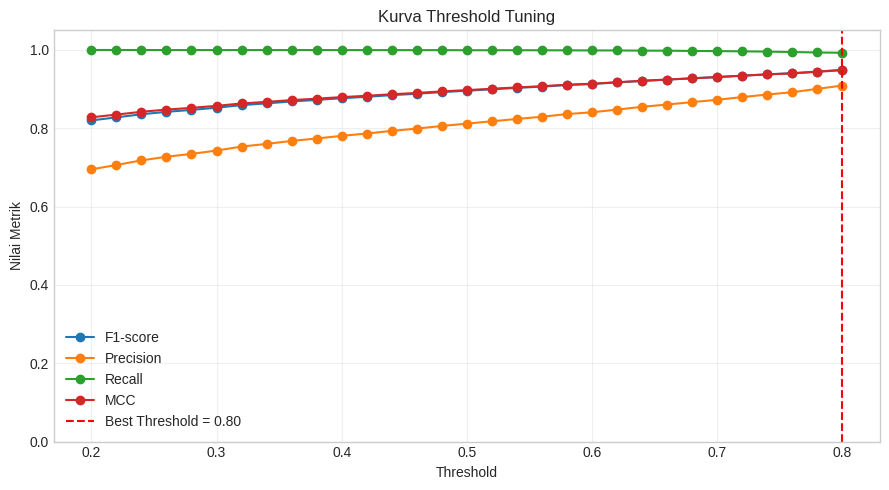
\includegraphics[width=5.51181in,height=3.0375in]{media/media/image16.png}

\phantomsection\label{_Toc228109344}{}Gambar 4. 7 Kurva Treshold Tuning

Berdasarkan Gambar 4.7, perubahan nilai threshold menghasilkan perubahan yang cukup jelas pada~F1,~precision,~recall, dan~MCC. Pola ini menunjukkan bahwa keputusan klasifikasi pada penelitian ini tidak cukup ditetapkan hanya berdasarkan probabilitas model, tetapi perlu disesuaikan melalui pemilihan ambang yang tepat. Oleh karena itu, tahap threshold tuning menjadi bagian penting dalam membentuk konfigurasi model final.

\subsection{Hasil Final Model Evaluation}\label{hasil-final-model-evaluation}

Setelah model final dan threshold terbaik diperoleh, eksperimen dilanjutkan ke evaluasi akhir pada data~test. Hasil evaluasi menunjukkan bahwa model final memiliki performa yang sangat tinggi pada beberapa metrik utama. Evaluasi ini memberikan gambaran mengenai kemampuan generalisasi model terhadap data yang tidak terlibat dalam proses pelatihan dan validasi.

Ringkasan metrik evaluasi akhir pada test set ditunjukkan pada Tabel 4.23.

\phantomsection\label{_Toc228109428}{}Tabel 4. 23 Final Metrics pada Test Set

\begin{longtable}[]{@{}
  >{\raggedright\arraybackslash}p{(\columnwidth - 10\tabcolsep) * \real{0.1931}}
  >{\raggedright\arraybackslash}p{(\columnwidth - 10\tabcolsep) * \real{0.1624}}
  >{\raggedright\arraybackslash}p{(\columnwidth - 10\tabcolsep) * \real{0.1595}}
  >{\raggedright\arraybackslash}p{(\columnwidth - 10\tabcolsep) * \real{0.1661}}
  >{\raggedright\arraybackslash}p{(\columnwidth - 10\tabcolsep) * \real{0.1595}}
  >{\raggedright\arraybackslash}p{(\columnwidth - 10\tabcolsep) * \real{0.1595}}@{}}
\toprule\noalign{}
\begin{minipage}[b]{\linewidth}\raggedright
\textbf{ROC-AUC}
\end{minipage} & \begin{minipage}[b]{\linewidth}\raggedright
\textbf{PR-AUC}
\end{minipage} & \begin{minipage}[b]{\linewidth}\raggedright
\textbf{F1}
\end{minipage} & \begin{minipage}[b]{\linewidth}\raggedright
\textbf{Precision}
\end{minipage} & \begin{minipage}[b]{\linewidth}\raggedright
\textbf{Recall}
\end{minipage} & \begin{minipage}[b]{\linewidth}\raggedright
\textbf{MCC}
\end{minipage} \\
\midrule\noalign{}
\endhead
\bottomrule\noalign{}
\endlastfoot
0,999876 & 0,996046 & 0,952511 & 0,913917 & 0,994507 & 0,951883 \\
\end{longtable}

Berdasarkan Tabel 4.23, model final menghasilkan~ROC-AUC~sebesar 0,999876, PR-AUC sebesar 0,996046, F1 sebesar 0,952511, Precision sebesar 0,913917, Recall~sebesar~0,994507, dan~MCC~sebesar~0,951883. Kombinasi nilai tersebut menunjukkan bahwa model tidak hanya memiliki kemampuan diskriminasi yang sangat tinggi, tetapi juga sangat baik dalam menyeimbangkan ketepatan dan kelengkapan deteksi klaim berisiko.

Untuk melihat hasil klasifikasi secara lebih konkret, confusion matrix model final ditunjukkan pada Gambar 4.8.

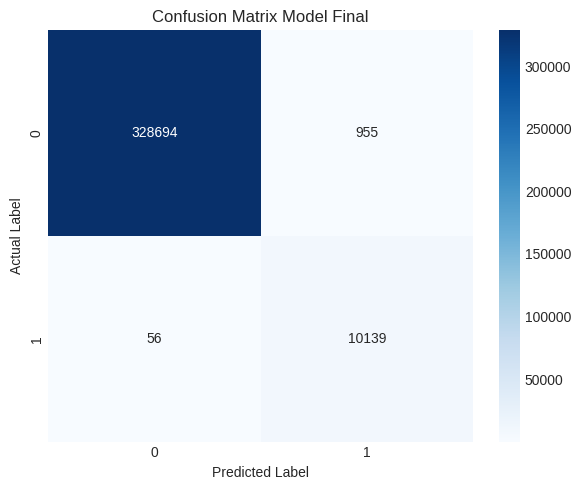
\includegraphics[width=5.51181in,height=4.65in]{media/media/image17.png}

\phantomsection\label{_Toc228109345}{}Gambar 4. 8 Confusion Matrix Model Final

Gambar 4.8 memperlihatkan bahwa model final mampu memisahkan sebagian besar klaim normal dan klaim berisiko secara tepat. Selain itu, untuk menilai kualitas pemeringkatan skor prediksi, kurva ROC dan kurva precision-recall ditunjukkan pada Gambar 4.9 dan Gambar 4.10.

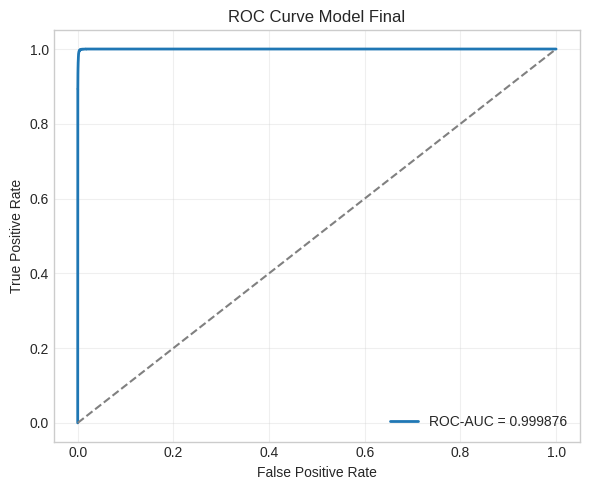
\includegraphics[width=4.93333in,height=4.09733in]{media/media/image18.png}

\phantomsection\label{_Toc228109346}{}Gambar 4. 9 ROC Curve Model Final

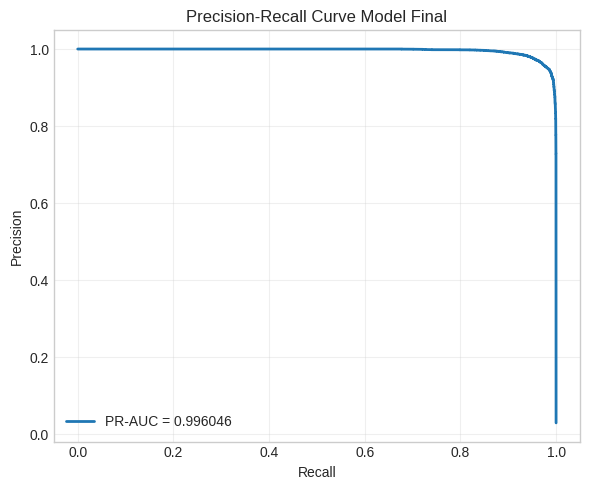
\includegraphics[width=4.87634in,height=4.05in]{media/media/image19.png}

\phantomsection\label{_Toc228109347}{}Gambar 4. 10 Precision-Recall Curve Model Final

Berdasarkan Gambar 4.9 dan Gambar 4.10, model final menunjukkan performa yang sangat baik dalam membedakan kelas dan memeringkat klaim berisiko pada berbagai nilai threshold. Hasil ini konsisten dengan tingginya nilai~ROC-AUC~dan~PR-AUC~yang diperoleh pada Tabel 4.23, sehingga evaluasi akhir menunjukkan bahwa konfigurasi model final memiliki kualitas prediksi yang sangat kuat pada data uji.

\subsection{Hasil Global Interpretability}\label{hasil-global-interpretability}

Setelah evaluasi performa selesai, eksperimen dilanjutkan ke tahap interpretabilitas global. Pada tahap ini, model final dibaca dari sisi fitur-fitur yang paling berpengaruh secara umum terhadap keputusan model. Hasil interpretabilitas global pada penelitian ini diperoleh melalui~feature importance,~SHAP, dan~PDP.

Feature importance~digunakan untuk melihat peringkat fitur dominan yang berkontribusi pada keputusan model final. Hasil ini memberikan gambaran awal mengenai fitur-fitur yang paling sering digunakan model dalam membedakan klaim normal dan klaim berisiko. Ringkasan visual feature importance model final ditunjukkan pada Gambar 4.11.

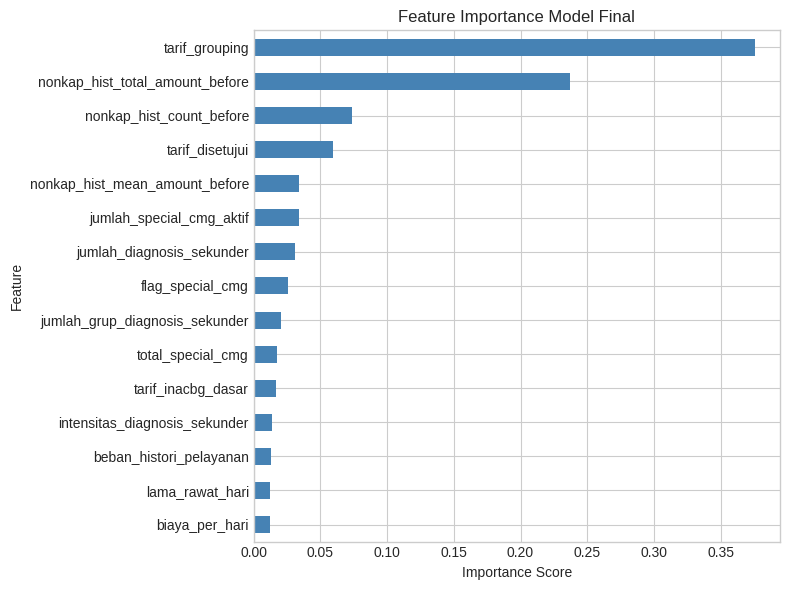
\includegraphics[width=5.51181in,height=4.11597in]{media/media/image20.png}

\phantomsection\label{_Toc228109348}{}Gambar 4. 11 Feature Importance Model Final

Gambar 4.11 menunjukkan peringkat fitur yang paling dominan dalam keputusan model final berdasarkan feature importance. Visualisasi ini memberikan gambaran awal mengenai variabel mana yang paling sering dimanfaatkan model untuk membedakan klaim normal dan klaim berisiko. Fitur-fitur yang berada pada peringkat atas didominasi oleh komponen biaya, histori layanan, dan karakteristik tarif, yang menunjukkan bahwa model sangat peka terhadap pola finansial dan histori utilisasi layanan dalam membaca sinyal risiko.

Selain itu,~SHAP summary plot~digunakan untuk membaca arah dan besar kontribusi fitur terhadap prediksi model. Gambar 4.12 menunjukkan bagaimana setiap fitur memberikan kontribusi yang berbeda terhadap peningkatan atau penurunan skor risiko model.

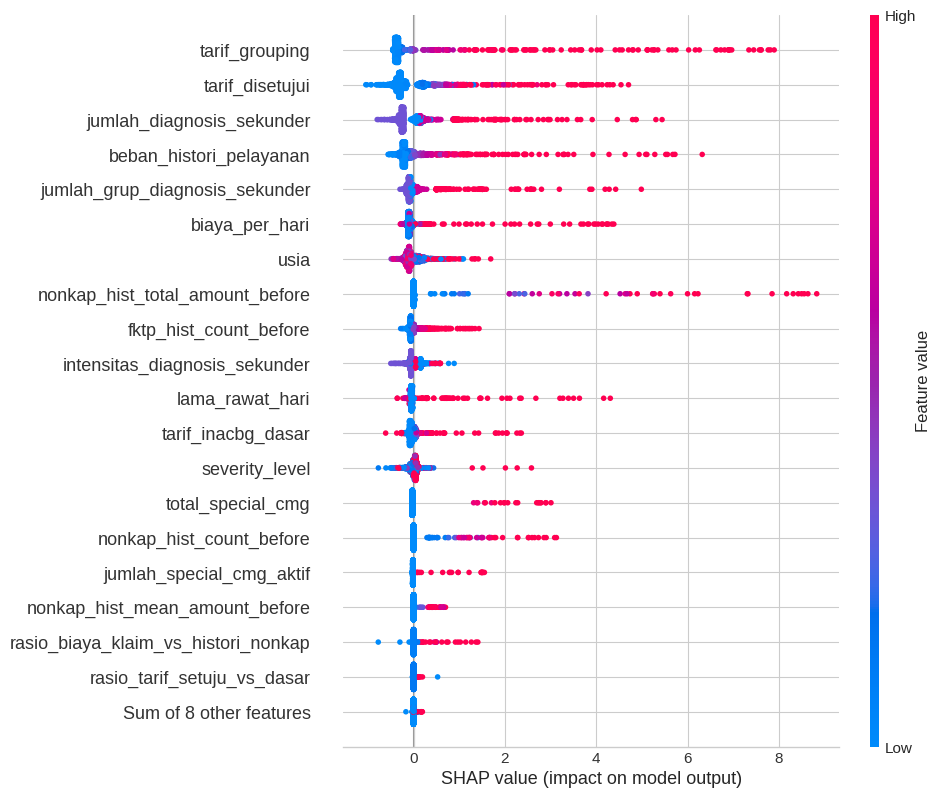
\includegraphics[width=5.51181in,height=4.68125in]{media/media/image21.png}

\phantomsection\label{_Toc228109349}{}Gambar 4. 12 SHAP Summary Plot

Untuk memperjelas pola pengaruh fitur dominan, eksperimen ini juga menghasilkan~PDP~untuk lima fitur teratas, yaitu~tarif\_grouping,~nonkap\_hist\_total\_amount\_before,~nonkap\_hist\_count\_before,~tarif\_disetujui, dan~nonkap\_hist\_mean\_amount\_before. Hasil tersebut ditunjukkan pada Gambar 4.13 sampai Gambar 4.17.

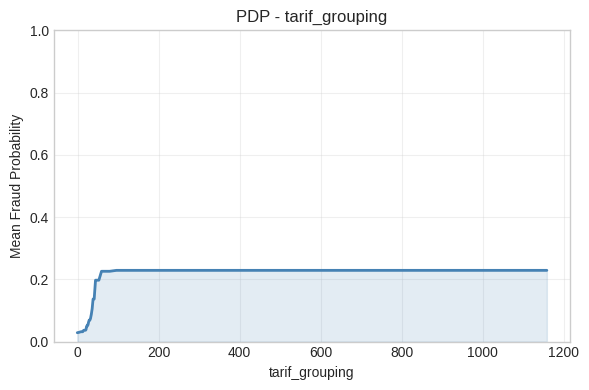
\includegraphics[width=5.51181in,height=3.64861in]{media/media/image22.png}

\phantomsection\label{_Toc228109350}{}Gambar 4. 13 PDP tarif\_groupping

Gambar 4.13 menunjukkan partial dependence plot untuk fitur tarif\_grouping. Kurva ini memperlihatkan bagaimana perubahan nilai tarif\_grouping berasosiasi dengan perubahan rata-rata probabilitas fraud yang diprediksi model. Pola tersebut menunjukkan bahwa tarif\_grouping menjadi salah satu penentu utama dalam pembacaan risiko klaim.

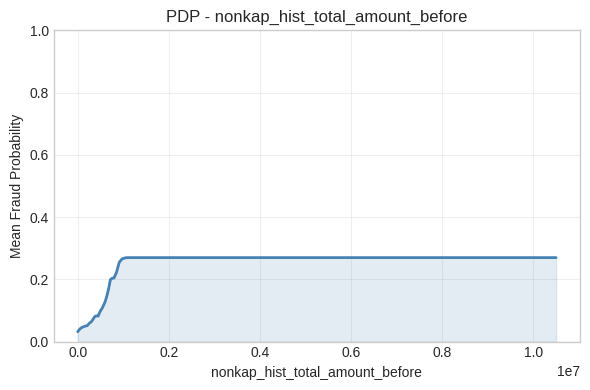
\includegraphics[width=5.51181in,height=3.64375in]{media/media/image23.png}

\phantomsection\label{_Toc228109351}{}Gambar 4. 14 PDP nonkap\_hist\_total\_amount\_before

Gambar 4.14 menunjukkan partial dependence plot untuk fitur nonkap\_hist\_total\_amount\_before. Hasil ini memperlihatkan bahwa histori total biaya nonkapitasi sebelum klaim turut memengaruhi probabilitas fraud, sehingga model tidak hanya membaca klaim saat ini, tetapi juga konteks histori pembiayaan sebelumnya.

Gambar 4.15 menunjukkan partial dependence plot untuk fitur nonkap\_hist\_count\_before. Pola ini menunjukkan bahwa frekuensi layanan nonkapitasi sebelum klaim memiliki kontribusi terhadap perubahan skor risiko, sehingga histori utilisasi layanan menjadi komponen penting dalam analisis.

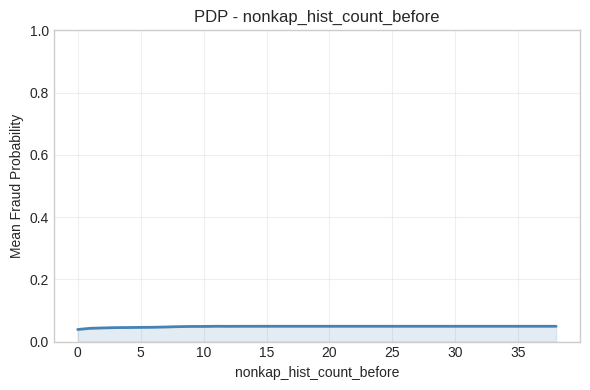
\includegraphics[width=5.51181in,height=3.64375in]{media/media/image24.png}

\phantomsection\label{_Toc228109352}{}Gambar 4. 15 PDP nonkap\_hist\_count\_before

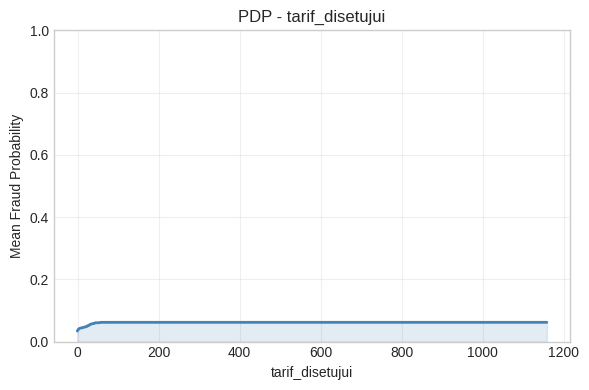
\includegraphics[width=5.51181in,height=3.64861in]{media/media/image25.png}

\phantomsection\label{_Toc228109353}{}Gambar 4. 16 PDP tarif\_disetujui

Gambar 4.16 menunjukkan partial dependence plot untuk fitur tarif\_disetujui. Sebaran pengaruh fitur ini memperlihatkan bahwa nilai biaya klaim yang disetujui memiliki hubungan yang cukup kuat dengan probabilitas fraud, meskipun pengaruhnya tidak selalu linear.

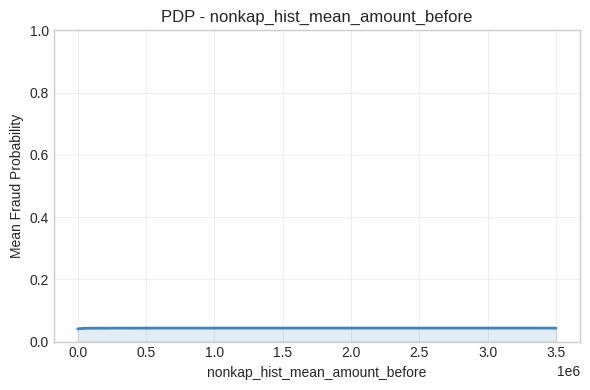
\includegraphics[width=5.51181in,height=3.64375in]{media/media/image26.png}

\phantomsection\label{_Toc228109354}{}Gambar 4. 17 PDP nonkap\_hist\_mean\_amount\_before

Gambar 4.17 menunjukkan partial dependence plot untuk fitur nonkap\_hist\_mean\_amount\_before. Hasil ini menegaskan bahwa rata-rata biaya histori nonkapitasi juga berperan dalam keputusan model, terutama ketika dibaca bersama fitur biaya dan histori lainnya.

Untuk merangkum hasil interpretasi global, Tabel 4.24 disajikan sebagai ringkasan teknik interpretasi, keluaran utama, dan fitur dominan yang muncul pada model final.

\phantomsection\label{_Toc228109429}{}Tabel 4. 24 Ringkasan Interpretasi Global

\begin{longtable}[]{@{}
  >{\raggedright\arraybackslash}p{(\columnwidth - 4\tabcolsep) * \real{0.1783}}
  >{\raggedright\arraybackslash}p{(\columnwidth - 4\tabcolsep) * \real{0.2325}}
  >{\raggedright\arraybackslash}p{(\columnwidth - 4\tabcolsep) * \real{0.5893}}@{}}
\toprule\noalign{}
\begin{minipage}[b]{\linewidth}\raggedright
\textbf{Teknik}
\end{minipage} & \begin{minipage}[b]{\linewidth}\raggedright
\textbf{Output Utama}
\end{minipage} & \begin{minipage}[b]{\linewidth}\raggedright
\textbf{Fitur Dominan}
\end{minipage} \\
\midrule\noalign{}
\endhead
\bottomrule\noalign{}
\endlastfoot
Feature Importance & Peringkat fitur utama & isi dari plot feature importance \\
SHAP & Arah dan besar kontribusi fitur & isi dari summary plot \\
PDP & Pola pengaruh lima fitur utama & tarif\_grouping,~nonkap\_hist\_total\_amount\_before,~nonkap\_hist\_count\_before,~tarif\_disetujui,~nonkap\_hist\_mean\_amount\_before \\
\end{longtable}

Berdasarkan Tabel 4.24, interpretasi global pada penelitian ini menunjukkan bahwa faktor biaya dan histori layanan memiliki kontribusi yang kuat dalam keputusan model final. Kehadiran fitur-fitur seperti~tarif\_grouping,~tarif\_disetujui, dan beberapa variabel histori layanan pada hasil~feature importance,~SHAP, dan~PDP~memperlihatkan bahwa model membaca risiko tidak hanya dari biaya absolut, tetapi juga dari hubungan antara komponen biaya dan pola layanan historis.

\subsection{\texorpdfstring{Hasil \emph{Local Interpretability} dan \emph{Top-Risk Claim Analysis}}{Hasil Local Interpretability dan Top-Risk Claim Analysis}}\label{hasil-local-interpretability-dan-top-risk-claim-analysis}

Setelah interpretasi global dilakukan, eksperimen dilanjutkan ke tahap interpretasi lokal pada klaim-klaim dengan probabilitas fraud tertinggi. Tahap ini bertujuan untuk menjelaskan alasan prediksi model pada level klaim individual. Dengan pendekatan ini, analisis tidak berhenti pada pola umum populasi, tetapi masuk ke level observasi individual yang paling relevan untuk ditelaah lebih lanjut.

Hasil eksperimen menunjukkan tiga klaim dengan probabilitas fraud tertinggi, yaitu 10241124V003022,~452460624V011711, dan~397950224V011829. Ketiga klaim tersebut memiliki probabilitas prediksi yang sangat tinggi dan kemudian dianalisis lebih lanjut menggunakan~LIME~untuk melihat fitur-fitur yang paling mendorong keputusan model. Ringkasan klaim berisiko tertinggi ditunjukkan pada Tabel 4.25.

\phantomsection\label{_Toc228109430}{}Tabel 4. 25 Top-Risk Claims

\begin{longtable}[]{@{}
  >{\raggedright\arraybackslash}p{(\columnwidth - 6\tabcolsep) * \real{0.0980}}
  >{\raggedright\arraybackslash}p{(\columnwidth - 6\tabcolsep) * \real{0.2763}}
  >{\raggedright\arraybackslash}p{(\columnwidth - 6\tabcolsep) * \real{0.2059}}
  >{\raggedright\arraybackslash}p{(\columnwidth - 6\tabcolsep) * \real{0.4198}}@{}}
\toprule\noalign{}
\begin{minipage}[b]{\linewidth}\raggedright
\textbf{Rank}
\end{minipage} & \begin{minipage}[b]{\linewidth}\raggedright
\textbf{ID Klaim}
\end{minipage} & \begin{minipage}[b]{\linewidth}\raggedright
\textbf{Fraud Probability}
\end{minipage} & \begin{minipage}[b]{\linewidth}\raggedright
\textbf{Faktor Utama}
\end{minipage} \\
\midrule\noalign{}
\endhead
\bottomrule\noalign{}
\endlastfoot
1 & 10241124V003022 & 1,0000 & histori nonkapitasi, tarif grouping, rasio tarif, tarif disetujui \\
2 & 452460624V011711 & 1,0000 & histori nonkapitasi, total special CMG, tarif grouping, special CMG \\
3 & 397950224V011829 & 1,0000 & tarif grouping, lama rawat, diagnosis sekunder, tarif disetujui \\
\end{longtable}

Berdasarkan Tabel 4.25, ketiga klaim teratas memiliki probabilitas fraud yang sangat tinggi dan didorong oleh kombinasi fitur yang berkaitan dengan komponen biaya, histori nonkapitasi, tarif grouping, dan beberapa indikator klinis tertentu. Hal ini menunjukkan bahwa keputusan model pada level lokal tetap konsisten dengan pola yang sudah terlihat pada interpretasi global.

Untuk memperjelas alasan prediksi pada ketiga klaim tersebut, hasil local explanation ditunjukkan pada Gambar 4.18 sampai Gambar 4.20.

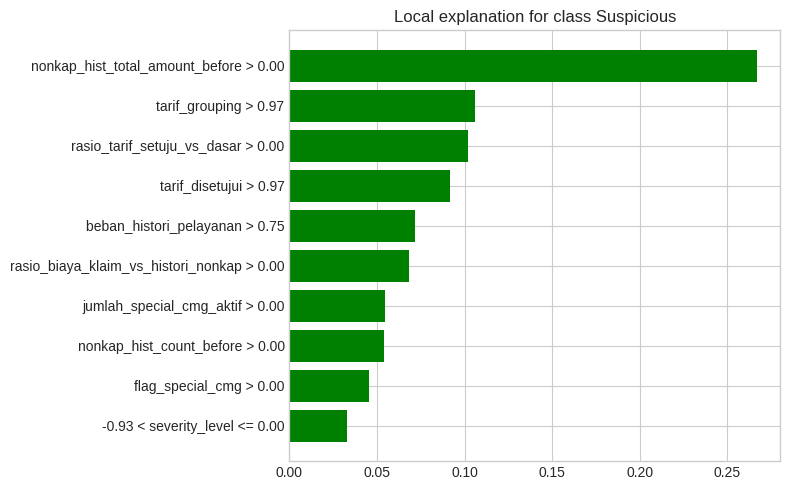
\includegraphics[width=5.51181in,height=3.41875in]{media/media/image27.png}

\phantomsection\label{_Toc228109355}{}Gambar 4. 18 Hasil LIME pada klaim 10241124V003022

Gambar 4.18 menunjukkan local explanation untuk klaim dengan probabilitas fraud tertinggi pertama. Hasil LIME memperlihatkan bahwa prediksi model terutama didorong oleh kombinasi histori nonkapitasi, tarif grouping, rasio tarif, dan tarif disetujui. Pola ini menunjukkan bahwa klaim tersebut dinilai berisiko karena memiliki karakteristik finansial dan histori layanan yang menyimpang dibandingkan populasi normal.

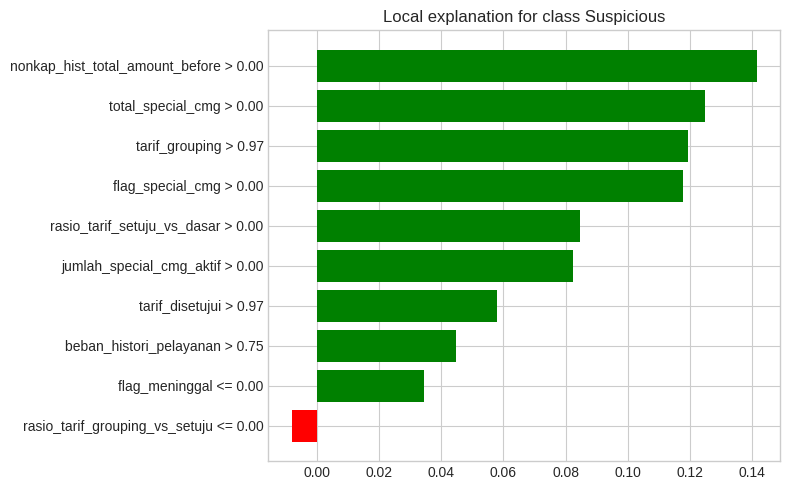
\includegraphics[width=5.51181in,height=3.41875in]{media/media/image28.png}

\phantomsection\label{_Toc228109356}{}Gambar 4. 19 Hasil LIME untuk pada 452460624V011711

Gambar 4.19 menunjukkan local explanation untuk klaim dengan probabilitas fraud tertinggi kedua. Pada klaim ini, faktor dominan yang mendorong skor risiko adalah histori nonkapitasi, total special CMG, tarif grouping, dan special CMG. Hal ini menunjukkan bahwa selain komponen biaya utama, tambahan biaya berbasis kompleksitas layanan juga berperan penting dalam keputusan model.

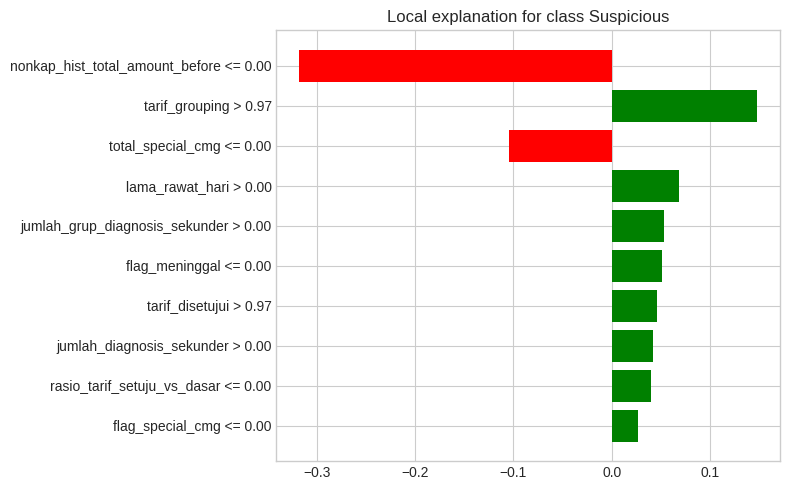
\includegraphics[width=5.51181in,height=3.41875in]{media/media/image29.png}

\phantomsection\label{_Toc228109357}{}Gambar 4. 20 Hasil LIME pada klaim 397950224V011829

Gambar 4.20 menunjukkan local explanation untuk klaim dengan probabilitas fraud tertinggi ketiga. Faktor yang paling berpengaruh pada klaim ini meliputi tarif grouping, lama rawat, diagnosis sekunder, dan tarif disetujui. Pola tersebut memperlihatkan bahwa model juga mempertimbangkan kombinasi aspek klinis dan finansial secara bersama dalam membaca risiko pada level klaim individual.

Berdasarkan Gambar 4.18 sampai Gambar 4.20, faktor pendorong utama pada ketiga klaim risiko tertinggi tidak sepenuhnya identik, tetapi memiliki pola umum yang serupa, yaitu dominasi komponen biaya dan histori layanan dalam mendorong skor risiko ke arah yang lebih tinggi. Dengan demikian, local interpretability pada penelitian ini menunjukkan bahwa model final tidak hanya kuat pada level populasi, tetapi juga dapat dibaca pada level klaim individual.

\subsection{Hasil Export Artifacts}\label{hasil-export-artifacts}

Tahap akhir dari eksperimen adalah penyimpanan artefak hasil. Artefak ini diekspor untuk memastikan bahwa keluaran utama dari pipeline dapat digunakan kembali untuk pelaporan, dokumentasi, dan verifikasi hasil eksperimen. Dengan adanya artefak tersebut, hasil eksperimen tidak hanya tersaji di lingkungan notebook, tetapi juga tersedia dalam bentuk keluaran yang terstruktur.

Artefak yang disimpan pada penelitian ini mencakup informasi model pemenang, hasil analisis threshold, daftar klaim berisiko tinggi, metrik evaluasi akhir, dan laporan interpretabilitas. Masing-masing artefak memiliki fungsi yang berbeda dalam mendukung pembacaan hasil pada Bab 4. Ringkasan artefak hasil yang diekspor ditunjukkan pada Tabel 4.26.

\phantomsection\label{_Toc228109431}{}Tabel 4. 26 Artefak Hasil yang Diekspor

\begin{longtable}[]{@{}
  >{\raggedright\arraybackslash}p{(\columnwidth - 4\tabcolsep) * \real{0.2542}}
  >{\raggedright\arraybackslash}p{(\columnwidth - 4\tabcolsep) * \real{0.4244}}
  >{\raggedright\arraybackslash}p{(\columnwidth - 4\tabcolsep) * \real{0.3214}}@{}}
\toprule\noalign{}
\begin{minipage}[b]{\linewidth}\raggedright
\textbf{Nama Artefak}
\end{minipage} & \begin{minipage}[b]{\linewidth}\raggedright
\textbf{Isi}
\end{minipage} & \begin{minipage}[b]{\linewidth}\raggedright
\textbf{Kegunaan}
\end{minipage} \\
\midrule\noalign{}
\endhead
\bottomrule\noalign{}
\endlastfoot
winner info & informasi winner branch, winner model, fitur, threshold & dokumentasi konfigurasi model final \\
threshold analysis & performa model pada berbagai threshold & dasar pemilihan threshold \\
top-risk claims & daftar klaim dengan probabilitas tertinggi & dasar analisis lokal \\
final metrics & metrik akhir model pada test set & pelaporan performa \\
laporan interpretability & keluaran SHAP, PDP, LIME, feature importance & menjelaskan hasil prediksi \\
\end{longtable}

Berdasarkan Tabel 4.26, artefak hasil pada penelitian ini tidak hanya berfungsi sebagai dokumentasi teknis, tetapi juga sebagai penghubung antara pelaksanaan eksperimen dan penulisan hasil.~winner info~dan~threshold analysis~mendokumentasikan konfigurasi model final,~top-risk claims~mendukung analisis lokal,~final metrics~mendukung pelaporan performa model, sedangkan laporan interpretabilitas membantu menjelaskan dasar keputusan model. Dengan adanya artefak-artefak ini, hasil eksperimen menjadi lebih mudah diverifikasi dan digunakan kembali pada tahap analisis.

\section{ANALISIS HASIL EKSPERIMEN}\label{analisis-hasil-eksperimen}

Subbab ini menganalisis hasil eksperimen yang telah disajikan pada Subbab 4.6. Analisis dilakukan secara paralel terhadap tahapan eksperimen, sehingga setiap keluaran utama tidak hanya ditampilkan sebagai hasil numerik atau visual, tetapi juga dijelaskan maknanya dalam konteks deteksi potensi fraud atau upcoding pada klaim JKN/BPJS. Dengan pendekatan tersebut, pembahasan pada subbab ini tidak mengulang hasil secara mentah, melainkan menafsirkan hasil tersebut dalam kaitannya dengan kualitas data, konfigurasi eksperimen, performa model, dan tujuan penelitian.

Analisis hasil eksperimen pada penelitian ini tidak hanya berfokus pada seberapa tinggi performa model, tetapi juga pada bagaimana model tersebut dibentuk, mengapa konfigurasi tertentu memberikan hasil yang lebih baik, dan apakah keluaran model dapat dijelaskan secara analitis. Oleh karena itu, subbab ini berfungsi untuk menghubungkan hasil eksperimen dengan logika metodologis penelitian serta menjelaskan kontribusinya terhadap tujuan penelitian secara utuh.

\subsection{Analisis Integrasi Claim-Centric dan Karakteristik Dataset}\label{analisis-integrasi-claim-centric-dan-karakteristik-dataset}

Hasil integrasi claim-centric pada Tabel 4.16 memperlihatkan bahwa satu klaim tetap dapat dipertahankan sebagai unit observasi utama meskipun data berasal dari beberapa sumber yang berbeda. Pendekatan ini penting karena model tidak hanya membaca klaim sebagai catatan biaya tunggal, tetapi sebagai entitas yang diperkaya oleh atribut peserta, diagnosis sekunder, dan histori layanan. Dengan demikian, struktur data akhir yang terbentuk lebih representatif untuk mendukung analisis risiko pada level transaksi klaim.

Integrasi multi-tabel juga memperkuat konteks analisis karena setiap sumber data memberikan kontribusi yang berbeda. Informasi dari kepesertaan memberikan konteks administratif dan demografis peserta, diagnosissekunder menambah kedalaman klinis, sedangkan fktpkapitasi dan nonkapitasi memberikan dimensi historis yang tidak tersedia pada klaim utama. Hasil integrasi seperti yang dirangkum pada Tabel 4.16 menunjukkan bahwa model pada penelitian ini dibangun di atas data yang lebih kaya daripada jika hanya bergantung pada tabel klaim mentah.

Karakteristik dataset yang ditunjukkan pada Tabel 4.10 dan Tabel 4.12 juga memperlihatkan bahwa data yang digunakan memiliki keragaman yang tinggi, baik dari sisi ukuran, tipe variabel, maupun dimensi informasinya. Variasi ini menjadi kekuatan sekaligus tantangan. Di satu sisi, keragaman tersebut memberikan sinyal yang lebih kaya untuk deteksi fraud. Di sisi lain, keragaman itu juga menuntut proses integrasi, standardisasi, dan seleksi fitur yang lebih ketat agar model tidak dibebani oleh variabel yang redundan atau kurang relevan.

Secara analitis, pendekatan claim-centric pada penelitian ini dapat dinilai lebih sesuai dengan tujuan deteksi fraud/upcoding karena fokusnya langsung berada pada klaim yang akan dievaluasi. Dengan struktur tersebut, eksperimen tidak hanya mampu membangun dataset pada level klaim, tetapi juga membentuk dasar yang lebih kuat untuk seluruh tahap pemodelan berikutnya.

\subsection{Analisis Pembentukan Pseudo-Label}\label{analisis-pembentukan-pseudo-label}

Dalam konteks penelitian ini, pseudo-label memiliki makna yang sangat penting karena berfungsi sebagai pengganti target pembelajaran pada kondisi ketika label fraud aktual tidak tersedia pada level klaim. Hasil pada Tabel 4.18 menunjukkan bahwa pseudo-label dibentuk melalui Isolation Forest dengan variasi contamination rate, sehingga eksperimen memiliki dasar yang lebih terukur dalam menentukan proporsi anomali yang akan digunakan sebagai target awal.

Nilai fraud ratio sekitar 3\% yang dihasilkan pada konfigurasi final menunjukkan bahwa klaim yang ditandai sebagai anomali memang hanya merupakan bagian kecil dari populasi. Secara analitis, hasil ini sesuai dengan karakter umum masalah fraud detection, di mana kejadian berisiko cenderung jarang dibandingkan dengan klaim normal. Artinya, pseudo-label yang terbentuk masih realistis dalam merepresentasikan sifat kasus yang hendak dideteksi, yaitu risiko fraud sebagai kelompok minoritas.

Perbandingan profil median antara klaim normal dan suspicious pada Gambar 4.6 memperlihatkan bahwa kelompok klaim anomali memiliki karakteristik yang berbeda secara cukup jelas dibandingkan Meioritas klaim. Klaim suspicious cenderung memiliki nilai median yang lebih tinggi pada beberapa indikator biaya dan layanan, sehingga pseudo-label yang terbentuk tidak bersifat acak. Pola ini menunjukkan bahwa Isolation Forest memang menangkap kelompok klaim yang memiliki struktur numerik berbeda dari populasi normal.

Dengan demikian, pseudo-label pada penelitian ini dapat dipahami bukan sebagai label fraud final, tetapi sebagai target awal yang cukup informatif untuk mendorong tahap supervised learning. Keberhasilan tahap ini penting karena seluruh proses benchmarking berikutnya bergantung pada kualitas target yang dibentuk pada tahap pseudo-labeling.

\subsection{Analisis Split, Preprocessing, dan Branch-Based Feature Selection}\label{analisis-split-preprocessing-dan-branch-based-feature-selection}

Hasil split dataset pada Tabel 4.19 menunjukkan bahwa distribusi label tetap konsisten pada subset train, validation, dan test, dengan rasio pseudo-label positif yang relatif sama pada ketiganya. Konsistensi ini penting karena menjaga agar pelatihan, validasi, dan evaluasi dilakukan pada distribusi kelas yang sebanding. Secara analitis, hasil ini menunjukkan bahwa proses pembagian data berjalan dengan baik dan tidak menimbulkan pergeseran distribusi yang dapat mengganggu pembacaan performa model.

Aspek berikutnya yang penting adalah kontrol terhadap data leakage. Pemisahan data lebih dahulu sebelum preprocessing dan pemodelan memastikan bahwa informasi dari data uji tidak bocor ke tahap pelatihan. Dalam penelitian ini, kontrol seperti itu menjadi krusial karena dataset sangat besar dan kaya fitur, sehingga tanpa pengendalian yang tepat, model berisiko memberikan performa yang tampak tinggi tetapi tidak benar-benar merepresentasikan kemampuan generalisasi.

Hasil branch-based feature selection pada Tabel 4.20 menunjukkan bahwa setiap branch menghasilkan jumlah dan karakter fitur yang berbeda. Dari hasil eksperimen, branch vif terbukti memberikan kombinasi paling efektif ketika dipadukan dengan model terbaik pada tahap benchmarking. Secara analitis, hasil ini menunjukkan bahwa pengurangan multikolinearitas memberikan manfaat yang nyata terhadap performa model. Dengan menekan redundansi hubungan linear antarfitur, branch vif memungkinkan model bekerja pada himpunan variabel yang lebih stabil dan lebih informatif.

Dengan demikian, hasil split, preprocessing, dan feature selection tidak boleh dipandang sebagai tahap teknis semata. Ketiganya justru berperan langsung dalam membentuk kualitas masukan model. Keberhasilan branch vif menunjukkan bahwa performa terbaik pada penelitian ini tidak hanya bergantung pada algoritma, tetapi juga pada kualitas struktur fitur yang digunakan.

\subsection{Analisis Benchmarking, Winner Selection, dan Threshold Tuning}\label{analisis-benchmarking-winner-selection-dan-threshold-tuning}

Hasil benchmarking pada Tabel 4.21 menunjukkan bahwa model final pada penelitian ini dipilih secara empiris berdasarkan performa aktual pada berbagai kombinasi branch dan algoritma. Hasil ini penting karena membuktikan bahwa konfigurasi terbaik tidak diasumsikan sejak awal, tetapi diperoleh melalui proses pembandingan yang sistematis. Dengan demikian, pemilihan model final benar-benar merupakan keluaran dari eksperimen, bukan keputusan yang ditetapkan secara apriori.

Dari seluruh kombinasi yang diuji, XGBoost pada branch vif menempati posisi terbaik dan kemudian ditetapkan sebagai winner, sebagaimana dirangkum pada Tabel 4.22. Hasil ini menunjukkan bahwa kombinasi antara model boosting dan himpunan fitur yang telah dikurangi multikolinearitasnya memberikan performa paling kuat pada data validasi. Keunggulan tersebut juga menegaskan bahwa struktur fitur memegang peran yang sama pentingnya dengan pemilihan algoritma.

Nilai threshold terbaik sebesar 0,80 memiliki arti penting secara analitis. Threshold ini menunjukkan bahwa klasifikasi akhir tidak dilakukan pada ambang probabilitas standar secara otomatis, tetapi melalui proses penyesuaian agar keseimbangan antara precision, recall, F1, dan MCC dapat dioptimalkan. Hubungan antar metrik terhadap perubahan threshold dapat dilihat pada Gambar 4.7, yang menunjukkan bahwa perubahan ambang klasifikasi menghasilkan perubahan performa yang cukup nyata.

Secara lebih spesifik, threshold yang lebih tinggi cenderung mendorong precision menjadi lebih baik, tetapi juga dapat menurunkan recall jika terlalu ketat. Sebaliknya, threshold yang lebih rendah cenderung memperbesar cakupan deteksi namun berpotensi meningkatkan false positive. Oleh karena itu, hasil pada Gambar 4.7 memperlihatkan bahwa threshold 0,80 dipilih karena memberikan titik keseimbangan yang paling sesuai dengan tujuan deteksi risiko pada penelitian ini.

\subsection{Analisis Kinerja Model Final}\label{analisis-kinerja-model-final}

Hasil evaluasi model final pada Tabel 4.23 menunjukkan bahwa model memiliki performa yang sangat tinggi terhadap target pseudo-label yang dibentuk pada tahap sebelumnya. Nilai ROC-AUC sebesar 0,999876 dan PR-AUC sebesar 0,996046 menunjukkan bahwa model sangat baik dalam membedakan klaim normal dan klaim berisiko serta dalam memeringkat probabilitas risiko pada kondisi data yang tidak seimbang.

Nilai F1-score sebesar 0,952511 menunjukkan keseimbangan yang sangat baik antara precision dan recall. Precision sebesar 0,913917 menunjukkan bahwa sebagian besar klaim yang ditandai berisiko memang relevan untuk diperhatikan lebih lanjut, sedangkan recall sebesar 0,994507 menunjukkan bahwa hampir seluruh klaim berisiko menurut pseudo-label berhasil ditangkap oleh model. Nilai MCC sebesar 0,951883 juga memperkuat bahwa performa model tetap tinggi ketika dievaluasi dengan metrik yang lebih seimbang pada distribusi kelas yang tidak merata.

Namun demikian, hasil ini perlu dibaca secara proporsional. Performa yang sangat tinggi pada penelitian ini menunjukkan kemampuan model dalam mempelajari dan memprediksi sinyal risiko yang dibentuk melalui pseudo-labeling, bukan secara langsung membuktikan kemampuan model dalam mengidentifikasi fraud aktual hasil audit resmi. Oleh karena itu, kekuatan utama model pada tahap ini adalah sebagai mekanisme penyaringan awal yang terukur, konsisten, dan siap digunakan untuk mendukung prioritisasi pemeriksaan klaim.

Dari sisi generalisasi, keberhasilan model pada data test tetap menunjukkan bahwa pipeline yang dibangun bekerja dengan baik pada data yang tidak terlibat dalam pelatihan dan validasi. Hasil pada Gambar 4.8, Gambar 4.9, dan Gambar 4.10 memperlihatkan bahwa model memiliki pemisahan kelas yang sangat baik pada confusion matrix serta kualitas pemeringkatan yang kuat pada kurva ROC dan precision-recall. Dengan demikian, model final dapat diposisikan sebagai alat bantu analitis yang kuat untuk mendukung proses verifikasi, dengan tetap menempatkan pembuktian fraud pada audit dan pemeriksaan lanjutan.

\subsection{Analisis Interpretabilitas Global dan Lokal}\label{analisis-interpretabilitas-global-dan-lokal}

Hasil interpretabilitas global pada Gambar 4.11, Gambar 4.12, dan Gambar 4.13 sampai Gambar 4.17 menunjukkan bahwa model final dipengaruhi secara kuat oleh fitur-fitur yang berkaitan dengan biaya, histori layanan nonkapitasi, dan komponen tarif. Temuan ini penting karena menunjukkan bahwa model tidak sekadar belajar dari satu indikator biaya tunggal, tetapi dari hubungan beberapa indikator finansial dan historis yang secara bersama-sama membentuk sinyal risiko.

Feature importance pada Gambar 4.11 memberikan gambaran awal mengenai fitur yang paling dominan pada keputusan model. Pembacaan ini menjadi lebih bermakna ketika dikombinasikan dengan SHAP pada Gambar 4.12, karena SHAP memperlihatkan arah dan besar kontribusi fitur terhadap prediksi. Dari kedua visual tersebut dapat dilihat bahwa beberapa fitur biaya, tarif grouping, serta histori layanan memiliki pengaruh yang kuat terhadap peningkatan skor risiko model.

PDP pada Gambar 4.13 sampai Gambar 4.17 memperdalam interpretasi tersebut dengan menunjukkan bahwa pengaruh fitur tidak selalu bersifat linier. Fitur seperti tarif\_grouping, nonkap\_hist\_total\_amount\_before, nonkap\_hist\_count\_before, tarif\_disetujui, dan nonkap\_hist\_mean\_amount\_before tidak hanya penting, tetapi juga memiliki pola pengaruh tertentu terhadap probabilitas fraud. Hal ini menunjukkan bahwa model menangkap hubungan yang lebih kompleks daripada sekadar hubungan sederhana antara biaya tinggi dan risiko tinggi.

Dari sisi interpretabilitas lokal, hasil pada Gambar 4.18 sampai Gambar 4.20 dan Tabel 4.25 menunjukkan bahwa tiga klaim dengan probabilitas fraud tertinggi memiliki pola risiko yang tetap konsisten dengan temuan global, yaitu dominasi faktor biaya, histori nonkapitasi, tarif grouping, serta beberapa indikator klinis tambahan. Namun demikian, masing-masing klaim tetap memiliki kombinasi faktor pendorong yang tidak sepenuhnya identik. Hal ini menunjukkan bahwa model final pada penelitian ini mampu menilai risiko secara individual, bukan hanya berdasarkan pola umum populasi.

Secara analitis, hubungan antara biaya, histori layanan nonkapitasi, tarif grouping, dan sinyal risiko menjadi salah satu temuan penting dalam penelitian ini. Temuan ini menunjukkan bahwa klaim berisiko tidak terbaca hanya dari tingginya biaya, tetapi dari kombinasi pola biaya, struktur tarif, dan riwayat layanan yang membentuk konteks ketidakwajaran. Bagi auditor atau verifikator, hasil interpretabilitas ini bernilai penting karena menyediakan alasan analitis di balik skor risiko, sehingga keluaran model dapat dibaca sebagai dasar prioritas pemeriksaan, bukan sekadar label prediksi yang berdiri sendiri.

\subsection{Keterkaitan Hasil Eksperimen dengan Tujuan Penelitian}\label{keterkaitan-hasil-eksperimen-dengan-tujuan-penelitian}

Secara keseluruhan, hasil eksperimen menunjukkan bahwa sistem yang dibangun pada penelitian ini berhasil mendeteksi potensi fraud atau upcoding pada level klaim. Keberhasilan tersebut terlihat dari terbentuknya pseudo-label yang informatif, pemilihan model final melalui benchmarking yang terukur, performa evaluasi yang sangat tinggi pada data uji, serta tersedianya interpretasi global dan lokal terhadap hasil prediksi. Dengan demikian, tujuan utama penelitian, yaitu membangun mekanisme analitis untuk menandai klaim berisiko, dapat dinyatakan tercapai.

Hasil eksperimen ini juga menunjukkan bahwa pipeline yang digunakan mampu bekerja secara konsisten dengan rancangan sistem yang telah dibangun sebelumnya. Alur mulai dari integrasi claim-centric, pseudo-labeling, branch-based feature selection, benchmarking multi-model, threshold tuning, hingga interpretabilitas terbukti dapat dijalankan secara utuh dan menghasilkan keluaran yang saling terhubung. Dengan kata lain, hasil eksperimen tidak berdiri sendiri, tetapi merupakan implementasi operasional dari kerangka sistem yang dirancang dalam penelitian ini.

Di samping itu, hasil penelitian menunjukkan bahwa sistem yang dibangun tidak hanya berfungsi untuk melakukan prediksi, tetapi juga mampu menjelaskan alasan di balik prediksi tersebut. Kehadiran feature importance, SHAP, PDP, dan LIME memperlihatkan bahwa keluaran model dapat dibaca dari dua tingkat sekaligus, yaitu tingkat populasi dan tingkat klaim individual. Hal ini penting karena pada domain klaim kesehatan, kemampuan menjelaskan hasil prediksi merupakan bagian yang sangat menentukan nilai praktis suatu sistem analitis.

Dengan demikian, jawaban terhadap tujuan penelitian dapat ditegaskan secara eksplisit sebagai berikut. Tujuan untuk membangun data analisis berbasis klaim telah tercapai melalui integrasi claim-centric. Tujuan untuk membentuk indikasi risiko awal telah tercapai melalui pseudo-labeling dengan Isolation Forest. Tujuan untuk menerapkan dan membandingkan beberapa model machine learning telah tercapai melalui benchmarking multi-model. Tujuan untuk menentukan konfigurasi keputusan terbaik telah tercapai melalui winner selection dan threshold tuning. Tujuan untuk menjelaskan hasil deteksi juga telah tercapai melalui interpretabilitas global dan lokal. Oleh karena itu, penelitian ini tidak hanya menghasilkan model klasifikasi, tetapi juga menghasilkan mekanisme analitis yang terstruktur, terukur, dan dapat dijelaskan untuk mendukung prioritisasi verifikasi klaim berisiko tinggi.

\emph{(Halaman ini sengaja dikosongkan)}
